%%% The main file. It contains definitions of basic parameters and includes all other parts.

%% Settings for single-side (simplex) printing
% Margins: left 40mm, right 25mm, top and bottom 25mm
% (but beware, LaTeX adds 1in implicitly)
\documentclass[12pt,notitlepage,a4paper,openright]{report}
\pagestyle{plain}

\PassOptionsToPackage{hyperfootnotes=false}{hyperref}

% fix pdfx
\usepackage{etoolbox}
% \makeatletter
% \@ifl@t@r\fmtversion{2021-06-01}%
%  {\AddToHook{package/after/xmpincl}
%    {\patchcmd\mcs@xmpincl@patchFile{\if\par}{\ifx\par}{}{\fail}}}{}
% \makeatother

\usepackage[usenames,dvipsnames,svgnames,table,rgb]{xcolor}
\usepackage[a-2u]{pdfx}
\usepackage{fontspec}
\usepackage[czech,english]{babel}
\usepackage{lmodern}
\usepackage{textcomp}
\usepackage{bbm}
\usepackage[defaultlines=4,all]{nowidow}

% Turn this on when needed:
%\usepackage{microtype}

\usepackage{graphicx}
\usepackage[twoside, inner=3.7cm, outer=2.9cm, top=2.6cm, bottom=3.4cm]{geometry}
\usepackage{thesis}
\usepackage[round]{natbib}
\usepackage{multirow}
\usepackage{arydshln} % dashed lines in tables
\usepackage{array}
\usepackage{amssymb,latexsym,pifont}
\usepackage{amsmath}
\usepackage{latexsym}
\usepackage{enumitem} % custom lists
\usepackage[normalem]{ulem} % underlining
\usepackage{setspace} % line spacing
\usepackage{varioref} % nice references (above/below)
\usepackage[above,section]{placeins} % avoid figures pushed at end of chapters
\usepackage{listings}

\usepackage{tabularx}
\usepackage{booktabs} % nicer lines in table
\usepackage{multicol}
\usepackage{tikz}
\usepackage{pgfplots}
\pgfplotsset{compat=1.18}
\usepackage{gnuplot-lua-tikz}
\usetikzlibrary{shapes.geometric}
\usepackage{epstopdf}
\usepackage{algorithmicx}
\usepackage{algorithm}
\usepackage{algpseudocode}
\usepackage{mathtools}
\usepackage{relsize}

% acronyms and glossaries
\usepackage[acronym, nomain]{glossaries}
\usepackage[shortcuts=ac]{glossaries-extra}
\makeglossaries
\preto\chapter{\glsresetall}

\setabbreviationstyle[acronym]{long-short}

\usepackage{subcaption} % sub figures in a fiture
\usepackage{standalone} % include standoalone tikz images
\usepackage{bibentry}

% hack bibentry command for list of publications
\makeatletter
\renewcommand\bibentry[1]{\nocite{#1}{\frenchspacing
     \@nameuse{BR@r@#1\@extra@b@citeb}}}
\makeatother

\hypersetup{
    colorlinks=false,
    pdfborder={0 0 0},
    unicode=true,
}

\input{acronyms}

% Czech babel conflicts with cline, hacky fix (http://tex.stackexchange.com/questions/111999/slovak-and-czech-babel-gives-problems-with-cmidrule-and-cline):
% - basically disables hyphenation in tables, but it's not used anyway so it doesn't matter
\preto\tabular{\shorthandoff{-}}
\preto\tikzpicture{\shorthandoff{-}}
%
%
\hyphenation{%
da-ta-sets
da-ta-set
} % -- custom hyphenation

% \setmainfont[Ligatures=Common]{Linux Libertine}
\setsansfont[Scale=MatchLowercase]{DejaVu Sans}
\setmonofont[Scale=MatchLowercase]{DejaVu Sans Mono}


\setstretch{1.1} % line spacing

\expandafter\def\expandafter\quote\expandafter{\quote\small} % smaller quotations font

% orphan & widow control
%\clubpenalty 10000
%\widowpenalty 10000

% gaps between text and footnotes
\def\footnoteskip#1{
  \renewcommand\footnoterule{
     \vspace{#1}
     \hrule width 0.4\columnwidth%
     \vspace{3pt}
}
}
\footnoteskip{0.8em}


\setcounter{tocdepth}{2}
\setcounter{secnumdepth}{2}

%% cutting down warnings
%\hfuzz=2pt
%\hbadness=10000

% force-ordering citations according to dummy keys
\newcommand{\dummybiborderkey}[1]{}

\input{macros}

\newcommand{\veryshortarrow}[1][3pt]{\mathrel{%
     \vcenter{\hbox{\rule[-.5\fontdimen8\textfont3]{#1}{\fontdimen8\textfont3}}}%
     \mkern-4mu\hbox{\usefont{U}{lasy}{m}{n}\symbol{41}}}}

\newcommand{\paperdisclaim}[1]{%
\begin{center}\begin{minipage}{0.9\textwidth}
\footnotesize\it #1
\end{minipage}\end{center}
}

\def\ignorecolumn#1\unskip{}

\definecolor{lightblue}{rgb}{0.6,0.8,1.0}
\definecolor{pastelgreen}{rgb}{0.65,0.8,0.4}
\definecolor{pastelyellow}{rgb}{1.0,0.8,0.5}

\title{Doctoral Thesis Template}

\def\fulldate{}
\author{Random Author}
\date{2022}
\dept{Institute of Formal and Applied Linguistics}
\supervisor{Ondra}
\studyprogram{Computer Science}
\studyfield{Computational Linguistics}


\begin{document}

%
%
%
\renewcommand{\thepage}{\roman{page}}
\selectlanguage{english}
\maketitle

\pagestyle{plain}
\normalsize
\setcounter{page}{2}

\cleardoublepage{}
\ \vspace{10mm}

\noindent \it

\vspace{\fill}
\noindent \rm
I declare that I carried out this doctoral thesis independently,
  and only with the cited sources, literature and other professional sources.

I understand that my work relates to the rights and obligations
  under the Act No.~121/2000 Coll., the Copyright Act, as amended,
  in particular the fact that Charles University has the right
  to conclude a license agreement on the use of this work as a school work
  pursuant to Section~60 paragraph~1 of the Copyright Act.

\vspace{2cm}
\noindent Prague, November 17, 1989 (TODO) \hspace{\fill}\theauthor % doplňte patřičné
                                                             % datum, jméno a
                                                             % příjmení

%%%   Do not forget to SIGN the printed book here!
%%%                  *********

\definecolor{darkgreen}{rgb}{0,0.5,0}
\definecolor{lightblue}{rgb}{0.7,0.9,1}
\definecolor{lblue}{rgb}{0.25,0.5,1}
\newcommand{\rewrite}[1] {
  {\color{blue}\textbf{TO BE REWRITTEN:} #1}
  }
\newcommand{\todo}[1] {
  {\color{red}\textbf{TODO:} #1}
  }
\newcommand{\VH}[1] {
  {\color{darkgreen}\emph{VH:} #1}
  }
 \newcommand{\kuba}[1] {
  {\color{darkgreen}\emph{Kuba:} #1}
  }
 \newcommand{\jindra}[1] {
  {\color{orange}\emph{Jindra:} #1}
  }
 \newcommand{\david}[1] {
  {\color{green}\emph{DM:} #1}
  }

\cleardoublepage{} % new page
\pagestyle{plain}

\addcontentsline{toc}{chapter}{English Abstract}

%\selectlanguage{english}
\begin{description}[leftmargin=7.5em,labelwidth=7em,labelindent=0em,labelsep=0.5em]
\item[Title:] \thetitle{}
\item[Author:] \theauthor{}
\item[Department:] \thedept{}
\item[Supervisor:] \thesupervisor{},\\ \thedept{}
\end{description}
\subsubsection{Abstract:}

This thesis focuses on developing and improving task-oriented dialogue systems design in the rapidly growing landscape of artificial intelligence and natural language processing.
We propose techniques that can substantially decrease development and deployment costs, motivated by the desire to make these systems more adaptable and scalable.
We introduce multiple approaches to achieving these goals, some of which we pioneer.

Firstly, we present a weakly supervised automatic data annotation pipeline that can transform raw data into a refined set of semantically coherent concepts, bypassing the need for exhaustive manual annotations and significantly streamlining the development process.

We also explore the largely uninvestigated field of latent variable models in task-oriented dialogue system modeling.
These models offer excellent capabilities with the potential to uncover the structure of behavioral patterns seen in the dialogue through inspection of the latent space and comparison with actions taken by the model.

Moreover, we harness the power of large pre-trained language models using in-context learning, following progress in the field.
Our proposed retrieval-augmented method performs well with merely a few training examples.
It shows great promise regarding human evaluation, implying a substantial leap in efficiently using computational resources to train conversational AI.
This brings us closer to more flexible and general-purpose systems.

In summary, the research presented in this thesis brings exciting innovations, uncovering new pathways in developing task-oriented dialogue systems.
It moves towards a future where dialogue systems can adapt, learn, and interact efficiently, potentially transforming how people interact with technology.

\begin{description}[leftmargin=7.5em,labelwidth=7em,labelindent=0em,labelsep=0.5em]
        %
\item[Keywords:] TODO add keywords such as: randomness, deep randomness, deep random processing (notice the nice black block marking the hbox overflow).
    %
\end{description}


\cleardoublepage{}
\addcontentsline{toc}{chapter}{Czech Abstract}
\selectlanguage{czech}
\begin{description}[leftmargin=7.5em,labelwidth=7em,labelindent=0em,labelsep=0.5em]
\item[Název práce:] TODO Český název práce TODO
\item[Autor:] \theauthor{}
\item[Katedra:] Ústav formální a aplikované lingvistiky
\item[Vedoucí práce:] \thesupervisor,\\ Ústav formální a aplikované lingvistiky
\end{description}

\subsubsection{Abstrakt:}

V této práci se soustředíme na vylepšení návrhu task-oriented dialogových systémů v době rychle se vyvíjejících technologií umělé inteligence.
Je žádoucí zajistit, aby systémy používající dialogové rozhraní byly snadněji adaptovatelné a rozšiřitelné.
Námi navržené techniky řeší oba tyto problémy a mohou výrazně snížit cenu vývoje i nasazení aplikací dialogových systémů.


Firstly, we present a weakly supervised automatic data annotation pipeline that can transform raw data into a refined set of semantically coherent concepts, bypassing the need for exhaustive manual annotations and significantly streamlining the development process.

We also explore the largely uninvestigated field of latent variable models in task-oriented dialogue system modeling.
These models offer excellent capabilities with the potential to uncover the structure of behavioral patterns seen in the dialogue through inspection of the latent space and comparison with actions taken by the model.

Moreover, we harness the power of large pre-trained language models using in-context learning, following progress in the field.
Our proposed retrieval-augmented method performs well with merely a few training examples.
It shows great promise regarding human evaluation, implying a substantial leap in efficiently using computational resources to train conversational AI.
This brings us closer to more flexible and general-purpose systems.

In summary, the research presented in this thesis brings exciting innovations, uncovering new pathways in developing task-oriented dialogue systems.
It moves towards a future where dialogue systems can adapt, learn, and interact efficiently, potentially transforming how people interact with technology.

\begin{description}[leftmargin=7.5em,labelwidth=7em,labelindent=0em,labelsep=0.5em]
%
\item[Klíčová slova:] TODO česká klíčová slova: nevim, nevim, nic
%
\end{description}

\selectlanguage{english}




\cleardoublepage{}
\ \vspace{10mm}

\addcontentsline{toc}{chapter}{Acknowledgements}
\subsection*{Acknowledgements}

{ TODO Here, you can thank anyone and say anything.

  \vspace{1\baselineskip}
  \noindent
  This is how I separated different kinds of thank-yous.

  \vspace{1\baselineskip}
  \noindent
  ... continued. }

\vfill


{\noindent\footnotesize %
  TODO Here, you can/should add stuff like: This work has been using language
  resources and tools developed and/or stored and/or distributed by the
  LINDAT/CLARIN project of the Ministry of Education, Youth and Sports of the
  Czech Republic (project LM2015071).%
}

\cleardoublepage{}
\addcontentsline{toc}{chapter}{Table of Contents}
\tableofcontents % automatically generated

\cleardoublepage{}
\renewcommand{\chapterheadstartvskip}{\vspace*{-10mm}} % chapter spacing
\setstretch{1.2} % line spacing

%
% TEXT START
%
\renewcommand{\thepage}{\arabic{page}}
\setcounter{page}{1}

\sloppy
% %%%%%%%%%%%%%%%%%%%%%%%%%%%%%%%%%%%%%%%%%%%%%%%%%%%%%%%%%%%%%%%%%%%%%%%%%%%%
\chapter{Introduction}%
\label{chap:intro}
Human language is a convenient and natural means of communication for human beings.
It is, therefore, desirable to implement an interface that mimics natural language and allows humans to interact with computers like they would with other human individuals.

To achieve this goal, we need to be able to transfer information between human users and the computer.
Humans most often use speech or written text to encode and transfer information, and some techniques deal with this kind of encoding, such as Automatic Speech Recognition (ASR), Optical Character Recognition (OCR), and Text-to-speech Synthesis (TTS).
However, to perform a meaningful dialogue, we need more than to mimic the interface.
The computer should be able to understand the meaning of utterances in the context and provide relevant responses.
In this work, we focus on this part of the problem, i.e. we do not care about encoding or decoding natural language in a signal such as speech.
Rather, we assume textual interfaces for both input and output.
Put simply, the task of a Dialogue System (DS) is to generate the correct natural language response \textit{r} given the natural language user utterance \textit{u} and context \textit{c}.
The dialogue is a \textit{turn-taking} conversation, i.e. participants (user and system) communicate in alternating \textit{turns}.

The ultimate goal is to construct a dialogue agent that provides meaningful responses to all kinds of questions, considering the conversation history.
Such an agent would effectively pass the Turing test, the holy grail for Artificial Intelligence.
The development of Large Language Models (LLMs) and their instruction tuning brings us close to achieving this goal.
Nevertheless, in many real-life cases, we do not need such complexity.
For example, we can take situated artificial agents who solely focus on achieving a certain well-specified goal, such as ordering food or reserving a flight ticket.

Dialogue systems promise a convenient means of communication between humans and computers.
They allow voice interaction, making it especially well suited for applications that should not disrupt attention, such as car control.
Systems capable of human-like conversation and accomplishing given tasks have huge potential to automate tech support processes and call centers or serve as personal assistants.

Despite some successful dialogue system deployments, dialogue systems still suffer from several drawbacks.
Usually, the DSs are tailored to specific applications, and applying them in other domains is hard.
Typically, the system is customized to handle a set of predefined domains with a high success rate.
A lot of effort goes into designing an ontology and handling domain-specific scenarios.
This results in bad scalability and inflexible applications.
Ideally, a system would learn common behavioral patterns required to finish the defined goal through conversational exchange successfully.
Given some description data, it could apply the learned knowledge to previously unseen domains and applications.
Although the LLMs make a huge step forward in this ability, they still might require finetuning and are not yet suitable for direct applications in the task-oriented world.

Another problem is that there seems to be a trade-off between interpretability and performance or scalability of the systems in the case of neural network-based models.
In most cases, the more complex and capable the model is, the harder it is to interpret its behavior and explain its decisions.

This thesis aims to propose solutions to some of these problems, especially in the task-oriented setting.
We now outline the main goals we want to achieve:
\begin{itemize}
    \item Make the task-oriented dialogue systems more scalable and easier to extend. As suggested, it is difficult to apply task-oriented systems on unseen domains for several reasons. (1) Extending the system is hard since it requires significant expert effort to design the schemas and annotate the data. In Chapter~\ref{chap:data_analysis}, we propose an automatic data analysis tool to gather information from dialogue corpora and suggest annotation schema without direct supervision.
    (2) It is difficult for the current system architectures to transfer the learned knowledge. To explore this phenomenon more, we conduct a series of experiments in Chapter~\ref{06:chap:lm-tod}. We also explore how to teach LLMs with a limited number of examples in Chapter~\ref{chap:llms}
    \item Enable the dialogue systems to leverage large unannotated data sets and train more robust models. There has not been much work on training task-oriented systems in an unsupervised way. We delve into our proposed models in Chapter~\ref{chap:modeling} and explore the usage of Pre-trained Language Models, which leverage large unannotated corpora, in Chapters~\ref{chap:lm-tod},\ref{chap:llms}.
\end{itemize}

Scalability and domain adaptation go hand in hand.
We focus on reducing the annotation needed to train a system and on knowledge abstraction to make transfer learning possible.
To leverage larger data sets, we explore unsupervised techniques that do not require annotation, making the data collection process substantially easier.

% %%%%%%%%%%%%%%%%%%%%%%%%%%%%%%%%%%%%%%%%%%%%%%%%%%%%%%%%%%%%%%%%%%%%%%%%%%%%



% %%%%%%%%%%%%%%%%%%%%%%%%%%%%%%%%%%%%%%%%%%%%%%%%%%%%%%%%%%%%%%%%%%%%%%%%%%%%
\chapter{Related Work}%
\label{chap:related}
% %%%%%%%%%%%%%%%%%%%%%%%%%%%%%%%%%%%%%%%%%%%%%%%%%%%%%%%%%%%%%%%%%%%%%%%%%%%%

\label{sec:relwork}
Because of varying use cases of DS, the architectures may vary a lot.
We thus introduce a classification of dialogue systems that reflects the expected capabilities.
There are multiple approaches to define a dialogue system taxonomy in the literature.
Here we introduce the widely used classification scheme \cite{jurafsky2000speech}.
\begin{enumerate}
    \item \textbf{Question Answering (QA)} - Although sometimes not mentioned in the context of dialogue systems, QA task can be seen as an instance of a simple conversation. The main task of a QA system is to provide answers to the user's questions.
    The topics may vary a lot and good understanding is essential for this task as well as knowledge representation.
    The dialogues are usually quite simple and often consist of just one question and the respective answer.
    \item \textbf{Task-oriented DS} - In this setting, the system's goal is to complete a task based on the user's instructions.
    The successful completion may depend on several attributes that the system has to learn from the user utterances.
    The system is also allowed to ask for additional information if needed and typically works with some external source of information such as database.
    Here the dialogues are usually much more complex than in the QA setting and dialogue context has to be taken into account.
    \item \textbf{Chit-chat} - In some cases, we might be interested in a system that is able to talk to the user casually and provide entertainment.
    Such systems might be used in combination with task-oriented systems to serve as human-like virtual assistants or possibly use the dialogue to advertise for products etc.
    The context and knowledge base are also important, but in most cases there is no well-defined task to be completed, so the evaluation is subjective.
\end{enumerate}

Another way of classifying the dialogues considers their domain of operation.
\textbf{Single-domain} systems are able to work only in one topic area, e.g. public transport or restaurant information, whereas \textbf{multi-domain} systems are able to handle multiple domains.
These types of systems aren't able to give meaningful answers outside of the domains that they're trained on.
A dialogue system is considered \textbf{open-domain} if it's able to have a conversation not limited to a predefined set of domains.
In practice, this is achievable only to some extent since the knowledge base of the program is always limited.
However, with internet access and smart information retrieval methods, the systems are able to cover tens of different domains.

Here we focus on the task-oriented DS and discuss it in more depth.
From the domain perspective, task-oriented DS are usually either single or multi domain systems, open-domain is not often the case.
We can see a task-oriented dialogue as a slot filling task.
That means we have a predefined set of semantic \textit{slots} that need to be filled with the right \textit{values}.
Each utterance in the task-oriented dialogue is considered an action that potentially changes the state of the conversation.
Such actions can be represented using \textit{Dialogue Acts (DA)}\cite{core1997coding}.
DA is a tuple consisting of user \textit{intent} (overall meaning of the sentence) and optionally also \textit{slot} and the corresponding \textit{value}.
In case that multiple slot values are present, all are considered to have the same intent.
An example dialogue with respective DA representation is depicted in Table \ref{fig:das}.
\begin{table*}[t]
\small
\setlength\fboxsep{2pt}
        \centering
        \begin{tabular}{rll}
        \textbf{\texttt{USER:}} & \textit{\texttt{I would like a cheap restaurant.}} & \textbf{\texttt{\colorbox{pastelyellow}{inform}(\colorbox{lightblue}{price}=\colorbox{pastelgreen}{cheap})}} \\
        \textbf{\texttt{SYSTEM:}} & \textit{\texttt{Golden plate is cheap.}} & \textbf{\texttt{\colorbox{pastelyellow}{inform}(\colorbox{lightblue}{name}=\colorbox{pastelgreen}{Golden plate})}} \\
        \hdashline[1.5pt/2pt]
        \textbf{\texttt{USER:}} & \textit{\texttt{What is the cuisine?}} & \textbf{\texttt{\colorbox{pastelyellow}{request}(\colorbox{lightblue}{cuisine})}} \\
        \textbf{\texttt{SYSTEM:}} & \textit{\texttt{They serve chinese food.}} & \textbf{\texttt{\colorbox{pastelyellow}{inform}(\colorbox{lightblue}{cuisine}=\colorbox{pastelgreen}{chinese})}} \\
        \hdashline[1.5pt/2pt]
        \textbf{\texttt{USER:}} & \textit{\texttt{Sounds good. Bye!}} & \textbf{\texttt{\colorbox{pastelyellow}{goodbye}()}} \\
        \textbf{\texttt{SYSTEM:}} & \textit{\texttt{Have a great day.}} & \textbf{\texttt{\colorbox{pastelyellow}{goodbye}()}} \\
        \end{tabular}
\normalsize
        \caption{Example of task-oriented dialogue in the restaurant reservation domain. Utterance representations as dialogue acts are depicted on the right. Intents are highlighted in orange, slot names in blue and respective values in green. Note that not all dialogue acts include slots and values}
    \label{fig:das}
\end{table*}
Most dialogue system modules for limited domains can be implemented by designing a set of rules and templates.
Such systems can yield satisfying results in some use cases, nevertheless, they are inflexible and generally not considered promising from the research point of view.
Therefore, we focus on data-driven approaches based on machine learning models.

\subsection{Modular architectures}
\label{sec:relwork-modular}
The traditional dialogue system implementation, especially for task-oriented dialogues, is based on modular architecture.
The modular system consists of several components connected to form a pipeline.
First, the Natural Language Understanding (NLU) module parses the utterance and creates structured representation.
Based on NLU outputs, the dialogue management module determines the next action.
Dialogue Management usually consists of the state tracker that updates state based on NLU outputs and the policy module that chooses the action.
Finaly, the language generation module is used to verbalize the chosen action.
\subsubsection{Natural Language Understanding (NLU)} The purpose of NLU is to extract the meaning of input utterances in natural language and transform it to a structured representation, i.e. dialogue acts.
Basically, the NLU module has three subtasks.
It has to determine the domain of the utterance, detect the user intent and capture any slot values, if present.
From the machine learning point of view, the intent and domain detection can be seen as a classification task and sentence-level classification can be utilized \cite{yaman2008integrative,schapire2000boostexter}.
The slot-value filling can be approached as a sequence tagging problem.
Many approaches have been proposed to tackle this issue, ranging from SVM \cite{shi2016recurrent} and HMM \cite{surendran2006dialog} based taggers to various neural models \cite{adel2016comparing, zhang2017position, mesnil2014using}.
Because of the similar nature of these three sub-tasks, it is reasonable to model them jointly.
Especially modeling the intent detection together with slot filling proved to be beneficial for the model performance \cite{zhang2017position, liu2016attention, xu2013convolutional}.
\subsubsection{Dialogue State Tracking (DST)} Dialogue state is used to keep track of the dialogue history, effectively providing the necessary context.
Dialogue State Trackers are used to update the state with correct values after each turn.
The most straightforward solution to this problem is a rule-based system that simply tracks the current slot values based on NLU.
However, the situation is usually more complicated.
We need to take into account a distribution of slot value probabilities and the update rules can be rather complex.
\citet{vzilka2013comparison} provides a comparison of different data driven models for dialogue state tracking.
Neural networks have also been used to model the distributions \cite{mrkvsic2016neural, zhong2018global} and deal with multiple domain handling \cite{rastogi2017scalable}.

\subsubsection{Dialogue Policy} The core component of the DS is the dialogue policy.
Its responsibility is to make the decision which action should the system take in each turn.
The policy decision can thus be framed as a classification task \cite{gavsic2013gaussian}.
Learning the policy just from the offline data might not produce robust policy due to low variability in the data.
Therefore, many works model the dialogue  as a partially observable Markov decision process \cite{gavsic2010gaussian, thomson2010bayesian}.
Reinforcement learning techniques are then applied to learn the policy and incorporate human  feedback \cite{peng2017composite, su2016line}.

\subsubsection{Natural Language Generation (NLG)} When the decision on a system action is made, the system needs to verbalize the action.
In other words, we need to create an utterance in natural language that expresses the information given in the system's underlying representation.
NLG is often realized with a set of handcrafted templates which are selected heuristically \cite{rudnicky_creating_1999}.
Variability of the generated utterances is limited and the scalability is poor.
Therefore corpus-based methods have been proposed \cite{oh2000stochastic, mairesse-young-2014-stochastic}.
Lately, neural network based systems were proposed as well \cite{wen-etal-2015-semantically, wen-etal-2016-multi}

\subsection{End-to-end architectures}
\label{sec:relwork-end-to-end}
The module-based approach is advantageous thanks to its good level of explainability.
In case of low performance, we can track the respective modules' outputs and find the source of problems.
On the other hand, error accumulation makes it difficult to recover from errors that were made by the modules early on in the pipeline.
Another disadvantage is the way how these systems are trained.
Each component requires specific data annotation, thus it can be difficult and costly to obtain a dataset suitable for training all of the components.
Also, the system design itself is more complicated since it requires implementation of multiple models.

Various end-to-end solutions have been proposed to address the drawbacks of modular system training.
This was made possible largely thanks to the growing popularity of Neural Networks (NN) and the backpropagation algorithm over the last decade.
NN form a family of models that naturally allow us to combine multiple models and train them using single training algorithm.
Therefore several solutions were proposed that implement the respective modules using neural network based models, interconnect them to form the pipeline and train them jointly \cite{li-etal-2017-end,wen-etal-2017-network}.
Although the end-to-end training improves scalability of the models, the proposed architectures still require multiple levels of data annotation for training.
To mitigate this problem, \citet{serban2016building} proposed a hierarchical end-to-end model that uses two levels of encoder-decoder Recurrent Neural Networks (RNN), one operating on dialogue turn level for keeping long-term context and one operating on word level for analyzing the current user input.
It does not follow the traditional pipeline scheme and thus does not require expert annotations.
However, it is not suitable for practical use in task-oriented DS in its raw form due to overall low performance and insufficient robustness.
The idea was further extended by \citet{williams2017hybrid} who introduced the \textit{Hybrid Code Networks}, an architecture that uses multiple utterance representations which are customizable by the developer.
Despite good performance and flexibility, the proposed model again required a non-trivial amount of data annotation.
\citet{lei2018sequicity} came with a novel idea to model the dialogue with an extended sequence-to-sequence model.
\label{sec:sequicity}
They use an encoder-decoder architecture based on RNN that generates a dialogue state prior to response generation.
They summarize the dialogue history in the RNN hidden state and use a system of copy mechanisms to be able to track the dialogue state.
The proposed dialogue state representation is greatly simplified and doesn't require explicit NLU input, thus the annotation process is significantly easier.

In recent years, the NLP word has witnessed a great success of attention based models (Transformers) \cite{vaswani2017attention} and their usage as pre-trained language models \cite{devlin-etal-2019-bert}.
In the area of dialogue systems, these models also show prominent results in the open-domain setting \cite{DBLP:journals/corr/abs-1901-08149} or for dialogue state tracking \cite{chao2019bert}.
The pretrained models are naturally utilizable for transfer learning, which proved to be useful in dialogue domain adaptation task \cite{shalyminov-etal-2019-shot}.
Recently, attention-based architecture was proposed that models latent dialogue actions \cite{bao2019plato}.

\subsection{Unsupervised and transfer learning methods}
\label{sec:relwork-unsup}
The research of methods that reduce the amount of supervision needed can be divided into two paradigms.
One direction of research tries to construct a method of unsupervised or weakly supervised data analysis, focusing on a certain part of the dialogue pipeline.
Such a method can provide artificial supervision for the supervised models introduced earlier.
The other option is to design a model that inherently doesn't need supervision or requires less annotation.

\subsubsection{Unsupervised analysis and labeling}
Various methods have been proposed to deal with NLU without explicit  supervision.
\citet{chen2016zero} first proposed a model for zero-shot user intent embedding prediction by training convolutional neural network that is trained to score the sentence-intent similarities.
Recently, \citet{shi2018auto} proposed an intent detection model with the use of sentence clustering based on sentence-level features.
They have applied their method successfully for the task of intent detection.

The idea of using semantic relations to perform language understanding in the unsupervised setting was proposed by \citet{heck2012exploiting}.
Here the authors use the Semantic Web \cite{berners2001semantic} which is a triple-based database of entity relations.
Their approach relies heavily on structured web pages for the target domain.
They exploit the structure to obtain semantic annotations in an unsupervised setting.

\label{sec:relwork-chen}
\citet{chen2014leveraging} combine the paradigms of semantic frame parsing with distributional semantics to perform unsupervised semantic slot induction.
The authors further improve their model in \citet{chen2015jointly} where they select the most prominent slot candidates using lexical knowledge graphs.

\citet{brychcin2016unsupervised} focused on modeling the dialogue as Markov decision process using HMMs.
By fitting the HMMs to the data, they explore the dialogue dynamics and assign Dialogue Acts to the HMM states.
\citet{shi2019unsupervised} took this approach one step further by using more complex model based on RNNs and Variational Autoencoders.
After fitting the model, they analyse the hidden state transitions and infer the dialogue structure from it.
\subsubsection{Modeling dialogues with less supervision}
Work regarding the usage of semi-supervised or unsupervised methods for the dialogue response generation task as a whole in the task-oriented setting has been limited so far.
One of the main challenges is to model the dialogue state with no supervision since it is by definition structured and might be quite complex.

The method proposed by \citet{jin2018explicit} builds on \citet{lei2018sequicity}'s sequence-to-sequence dialogue model (see Section~\ref{sec:sequicity}) by introducing a posterior regularization term in the loss function.
The model has two modules, a teacher and a student, to track the dialogue state and works in a semi-supervised way.
For supervised data, both tracker modules are trained with supervised classification loss.
For unsupervised data, teacher modeule can look at system responses, therefore it operates with more input information and makes more accurate predictions.
The student module is then trained to minimize the KL divergence loss.
The teacher module is conditioned on the system response, so it can't be used when the model is deployed, but it helps to train the student even with unlabeled data.

\citet{wen2017latent} introduced a model that learns latent intentions, bypassing the explicit dialogue state modeling.
\citet{zhao-eskenazi-2018-zero} approached the problem differently.
They designed a novel dialogue system model based on VAEs.
Their model uses supervised data from one domain to learn latent action representations.
Their recognition module is learned to map utterance representations to the same feature space as the action representations.
When transfering to another domain, the model needs only a small number of so-called seed responses to adapt.
Based on this idea, other works followed \citep{shalyminov-etal-2019-shot, huang2019mala}.


% %%%%%%%%%%%%%%%%%%%%%%%%%%%%%%%%%%%%%%%%%%%%%%%%%%%%%%%%%%%%%%%%%%%%%%%%%%%%
\chapter{Data analysis}%
\label{chap:data_analysis}
% %%%%%%%%%%%%%%%%%%%%%%%%%%%%%%%%%%%%%%%%%%%%%%%%%%%%%%%%%%%%%%%%%%%%%%%%%%%%
Task-oriented dialogue systems are widely used for various applications, such as customer service, personal assistance, and information retrieval. These systems aim to assist users in accomplishing specific tasks by engaging in a natural language conversation. In order to represent the meaning of user utterances, annotation based on \emph{slots} is commonly employed \cite{young_pomdp-based_2013}. Slots, which describe semantic concepts relevant to completing the task, serve as a means of capturing the user's desires as well as facilitating the system's communication with the user. Typical examples of slots include \emph{area}, \emph{price}, and \emph{address}, among others. By tracking slots and their values over the course of the dialogue, a dialogue system can maintain a \emph{dialogue state}, which allows it to effectively plan the next actions \cite{williams2013dialog}. The dialogue state represents explicitly all the important knowledge known to the system in a specific point in dialogue. Consequently, it can be utilized to communicate with external sources of information and data, such as databases, structured knowledge bases, or various APIs, in order to provide users with accurate and relevant information.

\section{Discovering dialogue slots}
Getting just raw, unlabeled, data for dialogue system training is not difficult, especially if we restrict the target domain.
In general it's sufficient to record some conversations happening either in real life or in artificial conditions. 
A requirement for dialogue state labels makes this process much more costly.
The sets of slots and their values typically need to be designed by domain experts.
This procedure consists of multiple tasks:
\begin{enumerate}
    \item Determine which concepts need to be captured
    \item Define them in consistent way
    \item Label the occurrences of these concepts in the training data.
\end{enumerate}
As mentioned, these steps require expert knowledge and sometimes non-trivial level of domain understanding.
Although we might design a system that does not rely on the usage of slots, both traditional pipeline systems \cite{young_pomdp-based_2013} and end-to-end task-oriented architectures \cite{wen2016network} typically require such annotation.
While some systems use implicit, latent state representation and do not require explicit labels \citep{serban2016building}, the behavior of such systems is hard to interpret or control, which can be crucial in practical applications.
Moreover, the use of slots enable communication with external interfaces, as discussed before.
There are several works aiming at keeping interpretability and reducing the annotation needs by automating it \citep{chen2014leveraging,chen2015jointly} or transferring annotation across domains \cite{zhao_zero-shot_2018,coope_span-convert_2020}, but they still require significant manual effort.
We present a novel approach to discovering a set of domain-relevant dialogue slots and their values given a set of dialogues in the target domain (such as transcripts from a call center).
Our approach requires no manual annotation at all in order to tag slots in dialogue data.
This substantially simplifies dialogue system design and training process, as the developer no longer needs to design a set of slots and annotate their occurrences in training data.
\subsection{Method overview}
We discover slots by analyzing outputs of generic domain-independent natural language taggers such as a semantic frame parser or a named entity recognizer (NER).
These models are able to detect important and relevant concepts in natural language utterances and subsequently group them using a set of pre-determined generic labels.
We call this approach \emph{weak supervision} since we are basically using labels as an input but these labels are noisy and do not correspond to the desired labels.
We use unsupervised clustering on top of annotation obtained by tagging models.
Nevertheless, the raw output of these models is not polished and cannot be used for the purpose of the dialogue system directly.
Let us consider an example given in Figure \ref{fig:tagged_example}.
\begin{figure}[h]
\centering
    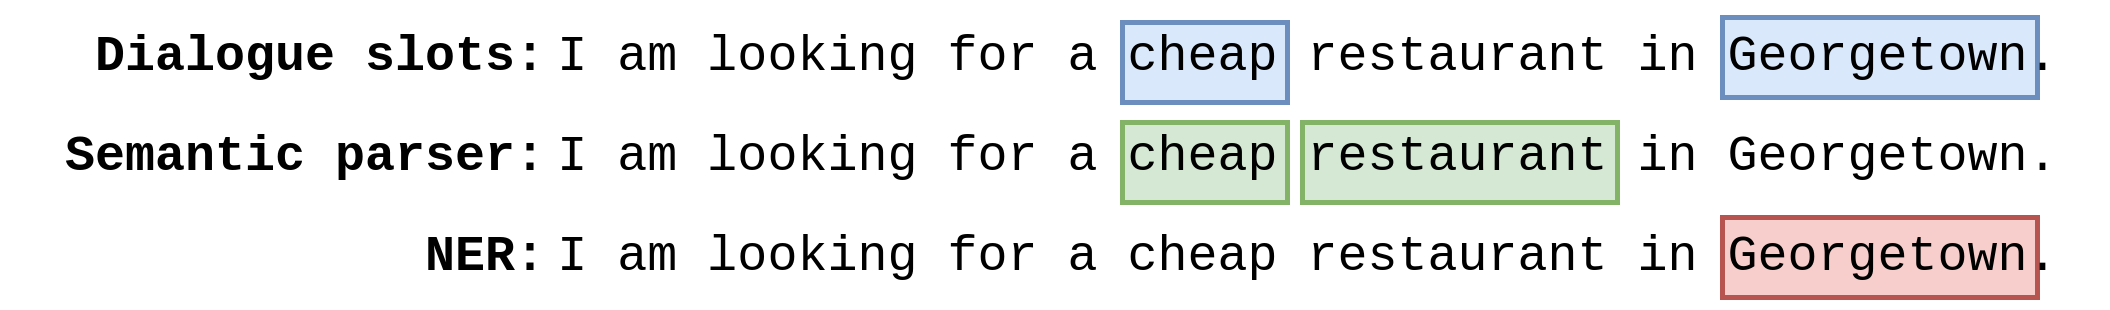
\includegraphics[width=0.8\textwidth]{images/tagging-example.png}
    \caption{An utterance from the restaurant recommendation domain tagged with generic semantic parser (green) and Named Entity Recognition system (red). We provide a comparison with ground truth dialogue slot labels (blue)}
    \label{fig:tagged_example}
\end{figure}
First we note that it helps to use multiple tagging models since some of the concepts might not be captured by a respective model.
The set of tagged words from all the sources covers all the dialogue slot values (\emph{cheap}, \emph{Georgetown}), however, it also contains irrelevant words (\emph{restaurant}).
This behavior is expected since the used tagging models are trained on generic open-domain data and therefore detect all semantic concepts mentioned in the utterances.
Therefore, in order to exploit the output of generic models we need to polish it and customize it to the specific domain.
Our method combines multiple sources of semantic labels and selects only relevant slot candidates.
Slots discovered by our approach can then be used to design a schema relevant to a specific domain.
Moreover, we train an independent, domain-specific tagger that can be used as a standalone component for natural language understanding.
A diagram describing our approach is depicted in Figure \ref{fig:discover_overall}.
\begin{figure}[h]
    \centering
    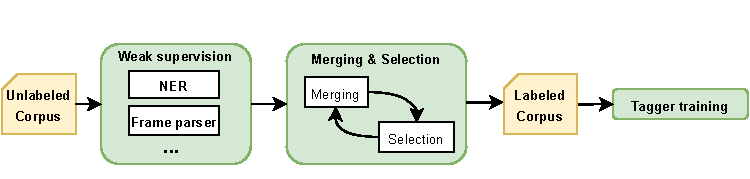
\includegraphics[width=0.9\textwidth]{images/weakly-supervised.pdf}
    \caption{Illustration of our pipeline. First, we analyze an unlabeled in-domain corpus with supplied domain-agnostic linguistic annotation models, such as a frame-semantic parser or NER. This results in slot candidates. Next, we iteratively merge and select slot candidates to obtain domain-relevant slots. Finally, we use the resulting slot labels in the corpus to train a neural slot tagger.}
    \label{fig:discover_overall}
\end{figure}

Next, we are going to describe the tagging models that were used in our experiments and go through all the stages of our method in detail.

\subsection{Tagging semantic concepts}
\label{03:tagging_concepts}
Our approach to selecting candidates for our method requires an initial pool of carefully chosen options that represent coherent concepts. This step is critical to ensure the effectiveness of our selection process. To achieve this goal, we strive to gather as many candidates as possible while still preserving the above constraint.
One of the key features of our method is its ability to merge several concepts into one, which means that we aim for high granularity and specificity in our input labels. As a result, we need to ensure that each candidate represents a unique concept that is distinguishable from others.

Given that we cannot rely on human annotations, we use an automatic procedure to gather the initial set of candidates.
In this procedure, we combine multiple sequence tagging models to label the input corpus.
The goal of this procedure is to identify words or phrases in the text that represent distinct concepts that can be used as candidate labels.
We can use any sequence tagging NLP model that meets the following criteria: (1) a set of words with the same label indicates semantically coherent, distinct concepts, (2) no additional annotation is needed, and (3) the model is domain-independent.
For our experiments, we chose two types of taggers to obtain the input tags: Frame Semantic Parser and Named Entity Recognition (NER).
By leveraging these models, we can quickly and accurately identify candidate labels that meet our criteria.
\begin{figure}[h!]
\centering
    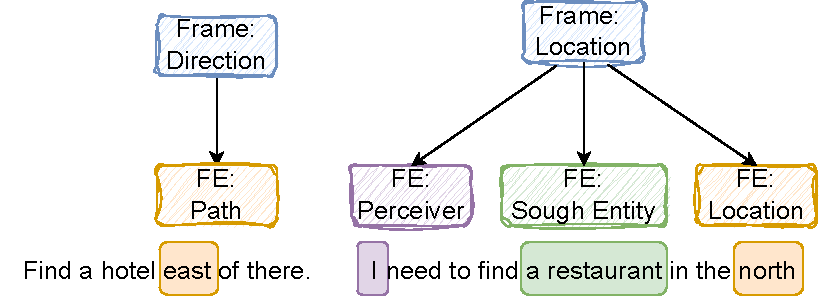
\includegraphics[width=0.8\textwidth]{images/framenet.pdf}
    \caption{An example of two Frames defined in the FrameNet dataset, together with core Frame Elements and respective instances. In this example we can see that a semantic concept representing the location of some place can be captured by multiple frames (\emph{Direction} and \emph{Location}). However, from the perspective of dialogue systems, these differences are negligible.Therefore we employ a merging strategy in our method.}
    \label{fig:framenet}
\end{figure}

\paragraph{Frame Semantic Parser} The parser is based on the FrameNet project \cite{baker1998berkeley}.
FrameNet is a lexical database of English language (although similar datasets exist in other languages) that aims to represent the usage of words in actual texts.
It contains over 200,000 utterances with more than 1,200 frames, each of which represent one semantic concept.
From the NLP perspective, it can be approached as a task of Semantic Role Labeling.
Each frame is formed by one or more frame elements which together form an instance of a certain semantic situation (e.g. \emph{Locale}, \emph{Offenses}, \emph{Size},...).
For the example of FrameNet instances see Figure \ref{fig:framenet}.
We take the individual Frame Elements as source for our slot candidates.
\paragraph{Named Entity Recognition} is a well-established task of labeling occurences of certain named entities in the input text data.
It fits well our requirements because the task is universal and the named entities definition is not specific to any particular domain.
\subsection{Selection of slot candidates}
\label{03:candidate_selection}
\begin{figure}[h]
    \centering
    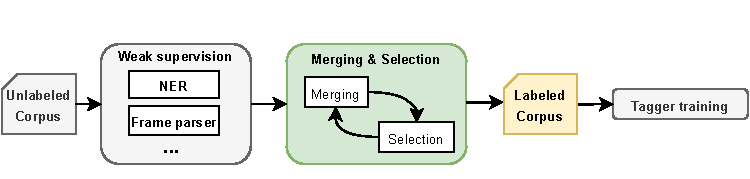
\includegraphics[width=0.9\textwidth]{images/merging.pdf}
    \caption{The selection step in our pipeline processes the input data and yields a set of slot candidates that should be relevant to the target domain.}
    \label{fig:candidate_selection}
\end{figure}
In the previous step, we obtained a superset of all the slot candidates by using weak supervision from the tagging models.
Subsequently, we need to identify domain-relevant slots based on candidates provided by the automatic annotation.
To achieve this, we design an iterative slot discovery procedure -- in each iteration, we: 
(1) merge similar candidates, 
(2) rank candidates' relevance and eliminates irrelevant ones.
Once no more frames are eliminated, the process stops and we obtain slot labels, which are used to train a slot tagger (see Section~\ref{03:training_tagger}).

We refer to the automatically tagged tokens as \emph{(slot) fillers}, and the tags are considered slot candidates.
In order to be able to select relevant candiates, we need to represent them in continuous space.
We use word embedding vectors and compute \emph{slot embeddings} $e(s_k)$ for each 
distinct slot candidate $s_k$ as word embedding averages over all respective slot fillers, weighted proportionally by filler frequency.
The slot embeddings need to be re-computed after each iteration due to the merging step.
We will now describe the individual steps.

\subsubsection{Candidate Merging}
\label{03:candidate_merging}
Since automatic annotation may have a very fine granularity, entities/objects of the same type are often captured by multiple slot candidates.
This is indeed the case for frame-semantic annotation, which we mostly use in our experiments.
With a frame parser, for instance, the frames \emph{Direction} and \emph{Location} both relate to the concept of \emph{area} which can be represented as a single slot.
We thus need to merge such similar slot candidates subsets $s_1 \dots s_n$ under a single candidate.
We further use syntactic parser to obtain dependency relations in which the slot fillers appear in the data and use this information to get more accurate similarity scores.
We measure similarity of slot candidates $s_1,s_2$ as:
\begin{equation}
    \text{sim}(s_1,s_2) = \text{sim}_{e}(e(s_1),e(s_2)) + \text{sim}_{\text{ctx}}(s_1,s_2)
\end{equation}
where $\text{sim}_{e}$ is a cosine similarity and $\text{sim}_{\text{ctx}}(s_1,s_2)$ is a normalized number of occurrences of $s_1$ and $s_2$ with the same dependency relation.
If the similarity exceeds a pre-set threshold $T_{\text{sim}}$, the candidates are merged into one.

\subsubsection{Candidate Ranking and Selection}
\label{03:candidate_select}
In this step we aim to eliminate irrelevant slot candidates and exclude them from the selection process.
To achieve this, we rank the slot candidates with respect to their importance computed from the data.
We hypothesize that different slots are likely to occur in different contexts (e.g., addresses are mentioned more when the system provides information to the user rather than stated by the user).
Some slots can occur rarely but still be relevant.
However, such rare slots would be overshadowed by more frequent slot candidates.
To preserve relevant slots that only occur in rarer contexts, we cluster the data into multiple clusters and then rank candidates within each cluster separately.
We consider candidates with a score higher than $\alpha$-fraction of a given cluster mean to be relevant and select them for the next iterations.
If a slot candidate is selected in at least one of the clusters, it is considered viable overall.

\paragraph{Clustering the data}
The purpose of data clustering step is to distinguish contexts in which the candidates appear.
We simplify the notion of context to the head verb connected with the respective slot filler word.
We process the data with a generic semantic role labeling tagger to obtain verb dependency relations.
Each occurrence of a filler is thus associated with a \emph{head verb} whose semantic argument the corresponding word is, if such exists. 
We then compute embeddings of the formed \emph{verb-filler} pairs as average of the respective token embeddings.
The pairs are then clustered using agglomerative (bottom-up) hierarchical clustering with average linkage according to cosine distance of their embeddings.
Note that fillers for the same slot candidate may end up in multiple clusters.
This does not mean that the respective slot candidate is split -- it is just ranked for relevance multiple times (with respect to multiple contexts).
The process stops when a predetermined number of clusters is reached.

\paragraph{Candidate Ranking criteria}
In order to rank the candidates, we need a function that computes a score for each candidate.
Since it is not clear how to compute the score, we use multiple attributes and combine them to compute the final score.
Specifically, we compute the following characteristics for each candidate:
\begin{itemize}[nosep,leftmargin=10pt]
    \item \textbf{Frequency} $\text{frq}(s)$ is used since candidates that occur frequently in the data are likely important.
    
    \item \textbf{Coherence} $\text{coh}(s)$ is the average pairwise similarity of all fillers' embeddings:
    \begin{equation}
        \text{coh}(s) = \frac{\mathlarger{\sum}_{(v,w) \in C^2_s}{d_{\cos}(e(v), e(w))}}{|C^2_s|}
    \end{equation}
    where $C^2_s$ is a set of all pairs of fillers for the slot candidate \emph{s}.
    We follow \citet{chen2014leveraging}'s assumption that fillers with high coherence, i.e., focused on one topic, are good slot candidates.
    
    \item \textbf{TextRank} \cite{mihalcea2004textrank} is a keyword extraction algorithm similar to the well-known PageRank todo : cite PageRank.
    It constructs a graph where nodes represent words and edges represent their co-occurrence.
    The dominant eigenvector of the adjacency matrix of this graph then gives the individual words' scores.
\end{itemize}
The final score is a simple sum of rankings with respect to all three scores.
For TextRank and frequency we use placeholder representing the slot candidate instead of the respective fillers.
Therefore we obtain scores relevant to candidates rather than the individual words.

\subsection{Training standalone tagger}
\label{03:training_tagger}
\begin{figure}[h]
    \centering
    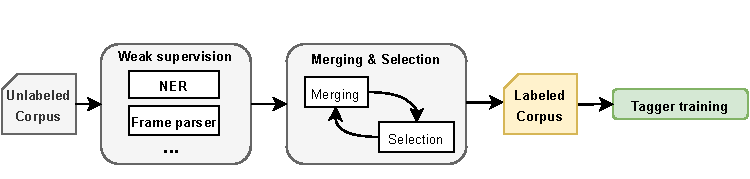
\includegraphics[width=0.9\textwidth]{images/tagging.pdf}
    \caption{After the set of slots is selected we assign the obtained labels to their occurrences in the data and use this labeled corpus to train a standalone tagger. }
    \label{fig:training_tagger}
\end{figure}
The motivation for training a tagger is two-fold.
First it's usage makes it possible to discard a dependency on the input taggers, thus the method's result is simpler to apply. 
Second, althoug the selection process can yield a good set of slots candidates, we experimentally discovered that the quality of the taggers used for initial input labeling can be insufficient, especially for some domains.
Therefore, using the merged and filtered slots directly may result in low recall since the original annotation models used as weak supervision are not adapted to our specific domain.
Therefore, we use the obtained labels to train a new, domain-specific slot tagger to improve performance.
The tagger has no access to better labels than those derived by our method; however, it has a simpler task, as the set of target labels is now much smaller and the domain is much narrower.

We model the slot tagging task as sequence tagging, using a convolutional neural network that takes word- and character-based embeddings of the tokens as the input and produces a sequence of respective tags \cite{lample2016neural}.\footnote{\url{https://github.com/deepmipt/ner}}
The output layer of the tagger network gives softmax probability distributions over possible tags.
In general, any sequence tagging model can be used, we choose a CNN-based tagger for its performance and a potential to easily customize the model.
Since our motivation is to improve recall, we add an inference-time rule -- if the most probable predicted tag is `O' (i.e., no slot) and the second most probable tag has a probability higher than a certain preset threshold, the second tag is chosen as a prediction instead.
Although this modification should improve recall, it also potentially tags irrelevant words and therefore it might harm the precision significantly and thus decrease the overall performance.
Nevertheless, we show in Section \ref{03:discovery_results} that the impact on precision is negligible while the recall can be indeed improved greatly. 

To improve the robustness of our model, 
we only use 10\% of the original in-domain training set to train the slot tagger model. The rest of the training set is used for a grid search to determine model hyperparameters (hidden layer size, dropout rate and $T_{\text{tag}}$ threshold). We choose the parameters that yield the best F1 score when compared against the automatic slot discovery results (i.e., no manual annotation is needed here, the aim is at good generalization).
\subsection{Experiments and results}
\label{03:discovery_results}
In this section we provide quantitative analysis of the results with respect to the NLU performance and quality of the discovered slots.
We also evaluate the application of this method as a module in end-to-end dialogue system model.
\paragraph{Datasets}
In order to evaluate our method in a complex way we use multiple datasets.
The datasets vary in several properties like number of domains or collection process.
This means we can compare the results on different data distributions and on tasks with different complexities.
Specifically, we use the following datasets in our experiments:
\begin{itemize}
    \item \textbf{CamRest676} (\textbf{CR}) \cite{wen2016network} has 676 dialogues, 2,744 user utterances, 4 tracked slots and 2 intents in the restaurant domain.
    \item \textbf{MultiWOZ} \cite{budzianowski2018multiwoz,eric2019multiwoz} is a multi-domain corpus; we picked two domains -- hotel reservation and attraction recommendation -- to form \textbf{WOZ-hotel} (\textbf{WH}) with 14,435 utterances, 9 slots, 3 intents and \textbf{WOZ-attr} (\textbf{WA}) with 7524 utterances, 8 slots and 3 intents respectively.\footnote{MultiWOZ contains more domains such as \emph{restaurant, train search, bus search}. However, we decided to not include these as they are nearly identical to the other domains we use.}
    \item \textbf{Cambridge SLU} \cite{henderson2012discriminative} (\textbf{CS}) contains 10,569 utterances and tracks 5 slots with 5 intents in the restaurant domain.
    \item \textbf{ATIS} (\textbf{AT}) \cite{hemphill_atis_1990} contains 4,978 utterances with 79 slots and 17 intents in the flights domain.\footnote{We used the ATIS data version from \url{https://www.kaggle.com/siddhadev/atis-dataset-from-ms-cntk}.}
\end{itemize}
\paragraph{3rd party models}
As sources of weak supervision providing slot candidates, we mainly use the frame semantic parsers \textit{SEMAFOR} \cite{das2010semafor} and \textit{open-sesame} \cite{swayamdipta2017frame} -- a union of labels provided by both parsers is used in all our setups. In addition, to explore combined sources on the named-entity-heavy ATIS dataset, we include a generic convolutional NER model provided by SpaCy.\footnote{\url{https://spacy.io}}
To provide features for slot candidate merging and selection, we use AllenNLP \cite{Gardner2017AllenNLP} for SRL
and FastText \cite{bojanowski2017enriching} as pretrained word embeddings.

\paragraph{Training details}
\begin{itemize}
    \item Slot merging and selection parameters were set heuristically in an initial trial run on the CamRest676 data and proved stable across domains.
    \item Slot tagger hyperparameters are chosen according to grid search on a portion of the training data.
    \item Since the models are rather small with regards to number of parameters, it is sufficient to use a regular desktop PC. In our experiments, we require about 4 GB of RAM, and we use Intel Xeon E5-2630 v4 CPUs. 
    \item Our slot candidate selection step takes roughly 1 hour.
    The tagger model is lightweight, with only 150k parameters. Its training requires 10-30 minutes, depending on the exact configuration and data size.
    \item The evaluation scripts are attached and described in the README file.
    \item We conduct hyperparameter search using a basic grid search algorithm. We tested hidden size values $\in [50,200]$, dropout $\in [0.5,0.85]$ and the threshold $T_{\text{tag}} \in [0.05,0.3]$. Therefore, we ran $4\times8\times6 = 192$ search trials.
    \item The best parameters were determined by tagger accuracy on the validation set: hidden\_size = 250, dropout = 0.7, $T_{\text{tag}} = 0.3$, $T_{\text{sim}} = 0.9$.
    \item Links to the data are included in the README file, we use \emph{train:validation:split} ratio equal to \emph{8:1:1}.
\end{itemize}

\paragraph{Evaluation Metrics}
We need a \textit{reference mapping} that maps our discovered slots to the ground truth labels to be able to evaluate the quality of the discovered concepts.
For evaluation, we construct a handcrafted  between our discovered slots and the respective ground-truth slots and intents.
his mapping is only needed for evaluation; it is not required by our method itself.
The mapping is domain-specific, but it is very easy to construct even for an untrained person -- the process takes less than 10 minutes for each of our domains.
It amounts to matching slots from the domain ontology against slots output by our approach, which are represented by FrameNet labels.
Most importantly, the mapping is \textbf{\emph{only needed for evaluation}}, not by our method itself.
We provide an example of such a reference mapping in Table \ref{03:ref_mapping}
\label{sec:app-ref-mapping}

\begin{table}[h!]
    \centering
    \small
    \begin{tabular}{rcl}
    \textbf{\emph{Ours-full} output} & & \textbf{CambridgeSLU ontology}\\\hline
     Expensiveness & $ \mapsto$ & Pricerange\\
     Origin + People\_by\_origin & $ \mapsto$ & Food\\
     Direction + Part\_orientational & $ \mapsto$ & Area\\
     Contacting + Artifact & $ \mapsto$ & Phone\\
     Locale\_by\_use & $ \mapsto$ & Type \\
     

    \end{tabular}
    \caption{An example of reference mapping between the output of \emph{Ours-full} represented by FrameNet labels (left) and ground-truth CambridgeSLU ontology (right).
    Frames merged by our method are shown on a single line, separated by “+”.
    }
    \label{03:ref_mapping}
\end{table}

For quantitative evaluation we use the following evaluation metrics:
\begin{itemize}[nosep,leftmargin=10pt]
    \item \textbf{Slot F1 score}: To reflect slot tagging performance, we measure precision, recall, and F1 for every slot individually.
    An average is then computed from slot-level scores, weighted by the number of slot occurrences in the data.
    We measure slot F1 both on standalone user utterances (slot tagging) and in the context of a dialogue system (dialogue tracking).
    \item \textbf{Slot-level Average Precision (AP)}. The slot candidates picking task is a ranking problem and we use the \textit{average precision} metric following \citet{chen2014leveraging}.
    Considering a ranked list of discovered slots $l = s_1, \dots, s_k, \dots, s_n$ we compute AP:
    \begin{equation}
        AP(l) = \frac{\sum_{k=1}^n P@k(l)\mathbbm{1}_k}{\mbox{\#\,mapped\ slots}}
    \end{equation}
    where $\mathbbm{1}_k$ is an indicator function that equals one if slot $k$ has a reference mapping defined and $P@k(l)$ is precision at $k$ of the ranked list $l$.
    \item \textbf{Slot Rand Index (RI)} is a clustering metric, used to evaluate slot candidate merging. RI is the proportion of pairs of slot candidates that are correctly assigned into the same or into different slots (following the reference mapping).\footnote{We compute RI on a union of labels that have a ground-truth slot mapping and all labels selected by our method. Labels without ground-truth mapping are assumed to form single-item “pseudo-slots”.}
    
    \item \textbf{Normalized Mutual Information (NMI)} is the mutual information between two clusterings normalized into the (0, 1) interval.
    Thanks to the normalization, it is suitable for comparing two clusterings with different numbers of clusters.

    
    \item \textbf{Intent Accuracy} is the percentage of slot occurrences assigned into the correct intent cluster under the reference mapping.
    \item \textbf{Dialogue Joint Goal Accuracy} calculates the proportion of dialogue turns where all user constraints (i.e., dialogue state summarizing slot values) are captured correctly \cite{mrkvsic2016neural}.
    
    \item \textbf{Dialogue Entity Match Rate} calculates the last turn's entity in each dialogue. It verifies if  a correct entity would be retrieved from the database using the final constraints \cite{wen2016network}.

\end{itemize}
For slot tagging and ranking evaluation, we sampled a random data order 50 times and performed 5-fold cross-validation for each permutation.
For the dialogue generation evaluation, we trained the models 100 times and used averaged results.
All results are given with 95\% confidence intervals.

\paragraph{Evaluated systems}
We test multiple variants of our system.
This gives us an idea about contributions of all the individual methods that we propose.
Here we give an overview of all the system variants:
\begin{itemize}[nosep,leftmargin=10pt]
    \item \textit{Ours-full} is the full version of our method (full annotation setup and trained slot tagger).
    \item \textit{Ours-nothr} does not use the recall-increasing second-candidate rule in the slot tagger.
    \item \textit{Ours-notag} excludes the slot tagger. This means that the outputs of input taggers are used directly to annotate the data.
    \item \textit{Ours-nocl} further excludes the clustering step; slot candidate ranking and selection is performed over all candidates together.
\end{itemize}
We also compare to previous work of \citet{chen2014leveraging},\footnote{We use our own reimplementation of their approach.}
This method is similar to the variant \textit{Ours-nocl}, but it does not merge similar frames and uses different ranking criteria.
Essentially, they use outputs of the input tagger after the selection step directly without any further processing.

To put our results into perspective, we also include two supervised models for comparison:
\emph{Tag-supervised} is the same model that we use as our slot tagger (see \ref{03:training_tagger}), but it is trained on supervised data with all ground truth labels available.
The other supervised baseline is called \emph{Dict-supervised}.
It uses a simple dictionary of slot fillers that is obtained directly from the training data.
We use straightforward word matching based on regular expressions to tag occurences of these values.


Apart from evaluation of the tagging performance w.r.t. NLU we are also interested in the intrinsic evaluation of the verb-slot pair clusters formed for slot ranking.
Specifically, we ask a question how well are these clusters formed and if they are meaningful.
We compare to gold-standard intent annotation with respect to the following baselines: (1) a majority baseline (assigning the most frequent intent class to all instances), and (2) a simple method that represents the utterances as averages of respective word embeddings and performs sentence-level intent clustering.
All the slots in a given utterance are then assumed to have the same intent.


\subsubsection{NLU}
\begin{figure}[h]
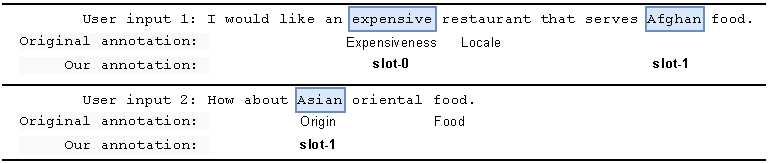
\includegraphics[width=1.0\textwidth]{images/label_example.pdf}
%\newtcbox{\bluebox}[1][]{nobeforeafter, tcbox raise base, shrink tight, sharp corners, extrude by=1mm, colback=blue!15, colframe=blue, #1}
%\newtcbox{\graybox}[1][]{nobeforeafter, tcbox raise base, shrink tight, sharp corners, extrude by=1mm, colback=gray!15, colframe=gray, #1}
%\small
%        \centering
%        \begin{tabular}{rl}
%        \hline
%        \texttt{user input 1:} & \textit{\texttt{I would like an \bluebox{expensive} \graybox{restaurant} that serves \bluebox{Afghan} food }} \\
%        \texttt{original annotation:} & \hspace{29mm} Expensiveness \hspace{4mm} Locale \hspace{33mm} - \\
        %\rowcolor{lightblue}
%        \texttt{our slot tagger:} & \bf\hspace{31mm} slot-0 \hspace{15mm} - \hspace{38mm}slot-1  \\
%        \hline
%        \texttt{user input 2:} & \textit{\texttt{How about \bluebox{Asian} oriental \graybox{food}?}} \\
%        \texttt{original annotation:} & \hspace{19mm} Origin \hspace{19mm} Food \\
        %\rowcolor{lightblue}
%        \texttt{our slot tagger:} & \bf\hspace{20mm}slot-0 \hspace{22mm} - \\
%        \hline
%        & ...
%        \end{tabular}
        \caption{A sample of a dialogue from CamRest676 data, with labels from a frame-semantic parser (middle) and our slot tagger (bottom).
        Although ``Afghan'' food is not in the frame parser output, our tagger was able to recognize it. The change in value for slot-1 (corresponding to food type) is successfully captured in the second utterance. This shows that our model can categorize entities (both ``Afghan'' and ``Asian'' relate to the same slot).}
    \label{fig:example}
\end{figure}
We evaluate our approach to slot discovery by comparing the resulting slot labels to gold-standard supervised slot annotation.
\paragraph{Slot tagging}\hspace{-3mm} is evaluated in Table \ref{table:slotfilling}.
\emph{Ours-full} (slot selection + trained tagger) outperforms all other approaches by a large margin, especially in terms of recall.
%\newtext{We note that the slot filling score is low even for the supervised version of our tagger.
%This is probably due to paraphrases and variants of slot values that can't be captured  well by the tagger.
The performance cannot match the supervised models, but it is not far off in some domains.\footnote{Note that our measurements of slot F1 only consider the `O' tag as negative (the average is computed over slots only). This results in lower numbers than those reported in literature \cite[cf.~e.g.][]{goo_slot-gated_2018}, but we believe that this reflects the actual performance more accurately.}
\citet{chen2014leveraging}'s method has a slightly higher precision, but our recall is much higher than theirs.
Note that \citet{chen2014leveraging} do not reduce the set of candidates, they only rank them so that a manual cut-off can be made.
In contrast, our method reduces the set of candidates significantly.
A comparison between \textit{Ours-notag} and \textit{Ours-full} shows that applying the slot tagger improves both precision and recall.
Tagger without the threshold decision rule (\textit{Ours-nothr}) mostly performs better than the parser; however, using the threshold is essential to improve recall.
Experiments on ATIS with NER as an additional source of annotation proved that our method can benefit from it.
As discussed above, the use of the trained tagging model is crucial to improve the recall of our method. In Figure~\ref{fig:tagger_comp}, we compare the results with and without the tagger. We change the value of prediction threshold and measure the number of cases in which the tagging model encounters more true positives, false positives or false negatives, respectively. As the results show, lowering the threshold increases the number of cases in which the tagger finds more correct slot values (and therefore improves recall), while it does not affect the number of false positives much (and therefore retains precision).
\begin{table}
        \centering
        \small
        \begin{tabular}{l|c|c|c|c}
        \hline
         \textbf{method} $\downarrow$ / \textbf{dataset}$ \rightarrow$ &  \textbf{CS} & \textbf{WH} & \textbf{WA} & \textbf{AT} \\
         \hline
        Tag-supervised$^\ast$ & $0.724 \pm .003 $ & $\pmb{0.742} \pm .008$ & $\pmb{0.731} \pm .002$ & $\pmb{0.848} \pm .003$ \\
         Dict-supervised$^\ast$ & $\pmb{0.753} \pm .005 $ & $\pmb{0.750} \pm .018$ & $0.665 \pm .003$ & $0.678 \pm .002$ \\\hline
        \bf weak supervision $\rightarrow$ & frames & frames & frames &  frames,NER \\\hline
         Chen et al. & $0.590 \pm .001 $ & $0.382 \pm .001$ & $0.375 \pm .001$ & $0.616 \pm .001$  \\\hdashline[0.5pt/2pt]
         %\hline
         Ours-nocl & $0.393 \pm .011 $ & $0.122 \pm .001$ & $0.266 \pm .008 $ & $ 0.677 \pm .002$ \\
         %\hline
         Ours-notag & $0.664 \pm .007$ & $0.388 \pm .002$ & $0.383 \pm .002$ & $ 0.648 \pm .003$ \\
         Ours-nothr & $0.569 \pm .031$ & $0.485 \pm .032$ & $0.435 \pm .002 $ & $0.698 \pm .004$\\
         %\hline
         Ours-full & $\pmb{0.692} \pm .008$ & $\pmb{0.548} \pm .004$ & $\pmb{0.439} \pm .001$ & $\pmb{0.710} \pm .002$ \\
         \hline
        \end{tabular}
                 
        \caption{F1 score values with 95\% confidence intervals for slot tagging performance comparison among different methods. The measures are evaluated using a manual slot mapping to the datasets' annotation, which is not needed for the methods themselves. $^\ast$Note that supervised setups are not directly comparable to our approach.
        \label{table:slotfilling}
        }
\end{table}

\paragraph{Error analysis:}
We conducted a manual error analysis of slot tagging to gain more insight about the output quality and sources of errors.
In general, we found that the tagger can generalize and capture unseen values.
\begin{figure}
    \centering
    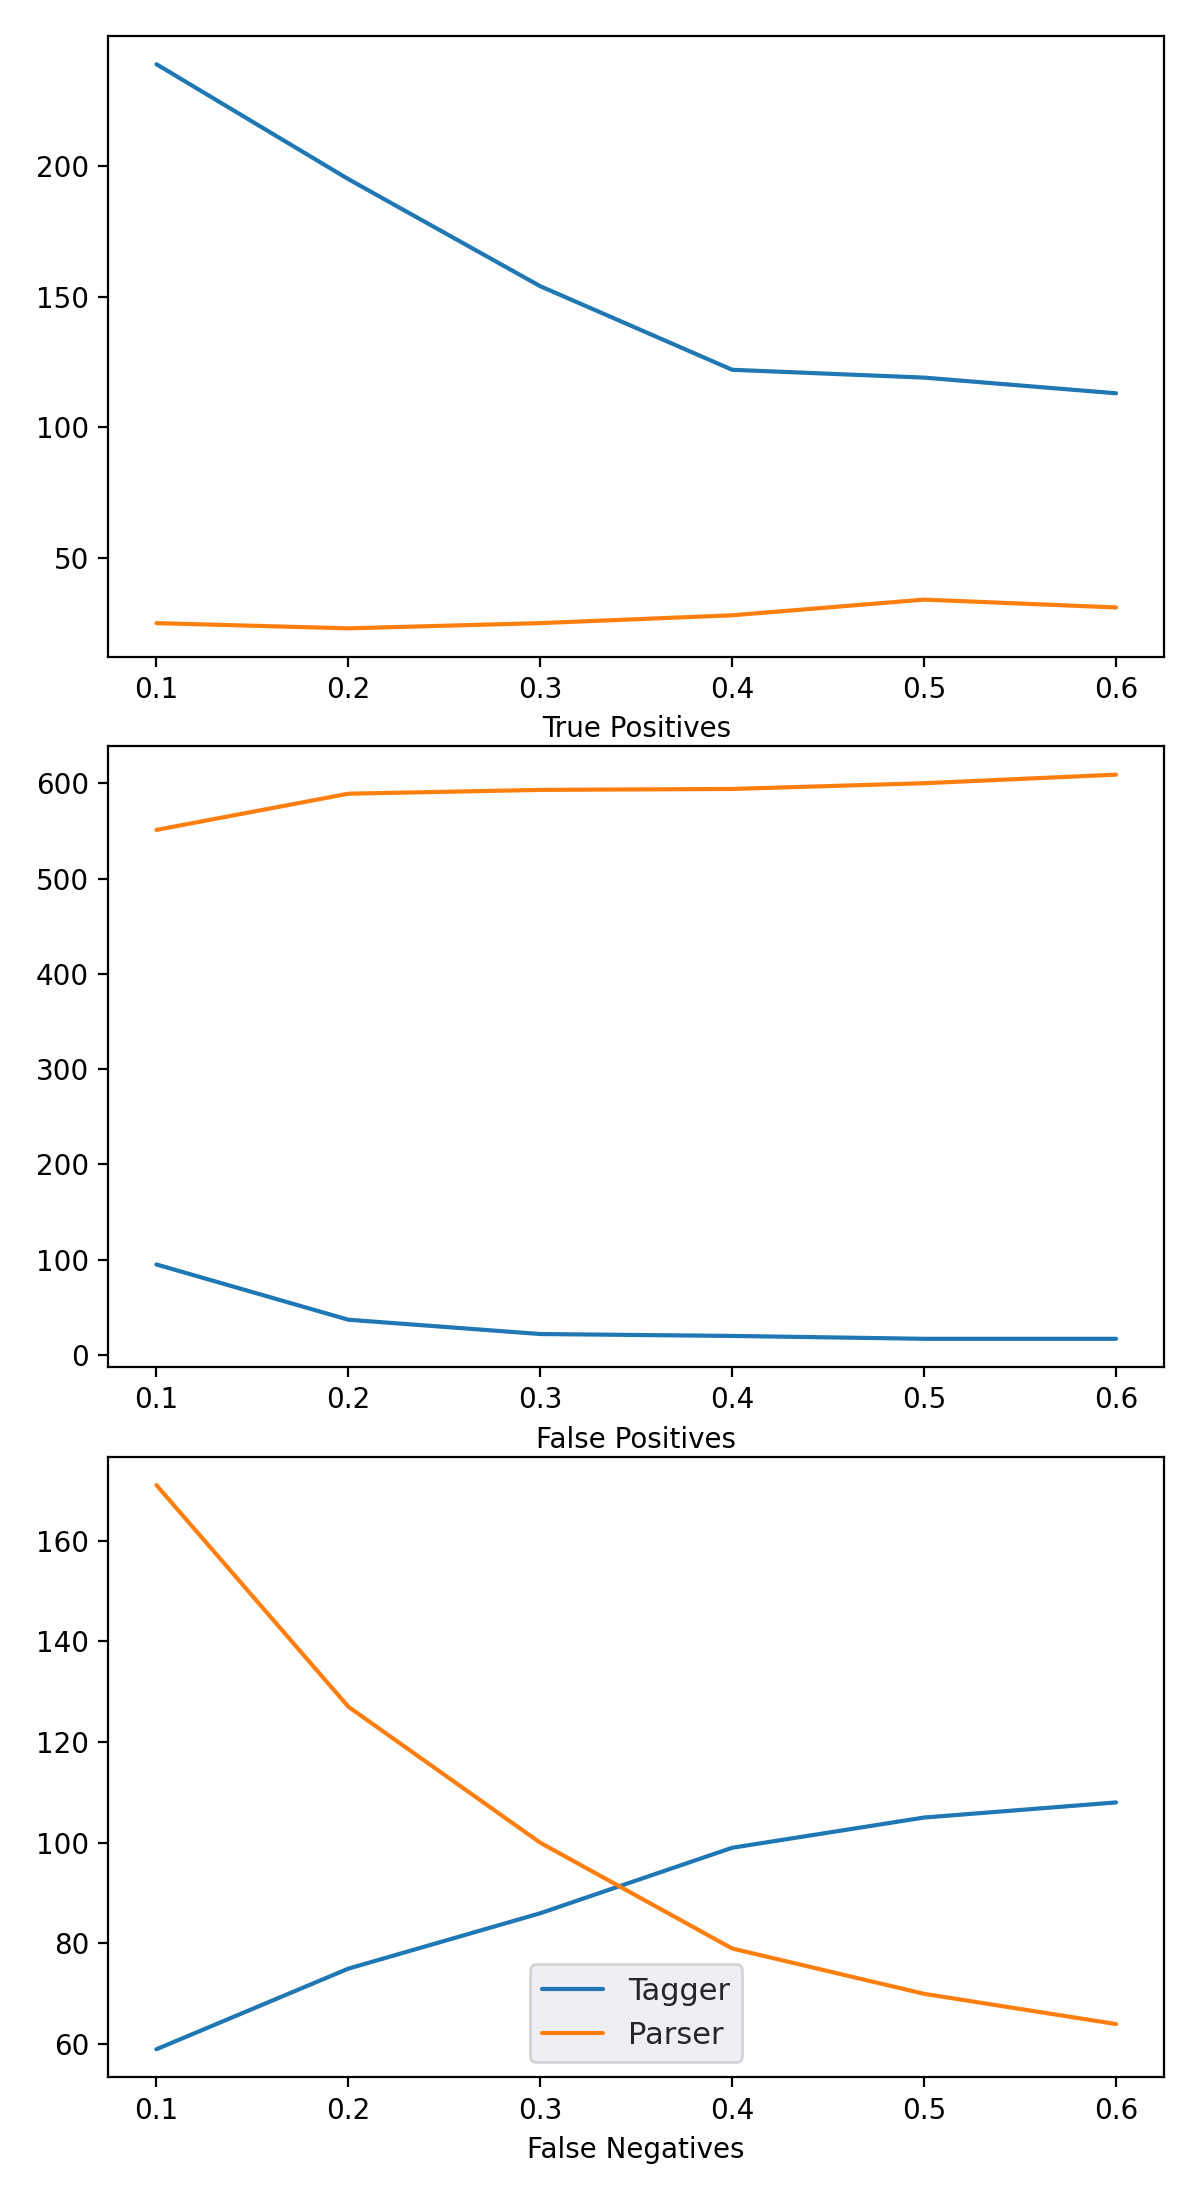
\includegraphics[width=0.45\textwidth]{images/slots.png}
    \caption{The comparison of outputs of our tagger and the parser. The plots show a number of cases in which the respective approach encounters more TPs, FPs or FNs than the other.}
    \label{fig:tagger_comp}
\end{figure}

One source of errors is the relatively low recall of the frame-semantic parsers used.
We successfully address this issue by introducing the slot tagger, however, many slot values remain untagged.
This is expected as our method's performance is inherently limited by the input linguistic annotation quality.
Another type of errors is caused by the candidate merging procedure (see also below).
Due to frequent co-occurrence, it might happen that two semantically unrelated candidates are merged and therefore some tokens are wrongly included as respective slot fillers.
Nevertheless, the merging step is required in order to obtain a reasonable number of slots for a dialogue domain.

Our approach does leave some room for improvements, especially regarding the consistency of results across different slots, which can be imbalanced.
\begin{table}[h]
    \centering
    \small
    \begin{tabular}{l|ccccccccc}
    \hline
    \textbf{dataset} & \textbf{price} & \textbf{area} & \textbf{request} & \textbf{type} & \textbf{food} & \textbf{day} & \textbf{people} & \textbf{stars} & \textbf{stay}
    \\ \hline
    \textbf{CR} & 0.54 & 0.76 & 0.76 & -- & 0.59 & -- & -- & -- & -- \\
    \textbf{CS} & 0.63 & 0.84 & 0.48 & 0.81 & 0.64 & -- & -- & -- & -- \\
    \textbf{WH} & 0.21 & 0.52 & 0.11 & 0.13 & -- & 0.15 & 0.82 & 0.82 & 0.34 \\
    \hline
    \end{tabular}
    
    \caption{Per-slot F1 scores of the \emph{Ours-full} method evaluated on selected datasets with slot intersection. For some slots the performance varies a lot among datasets due to different ranges of values and contexts. The measures are evaluated using a manually designed slot mapping to the datasets' annotation, which is not needed for the methods themselves.}
    \label{table:slotfilling_detail}
\end{table}

\paragraph{Slot candidate ranking}\hspace{-3mm} results are given in Table~\ref{table:avg-precision}.
Our pipeline significantly outperforms \citet{chen2014leveraging}'s approach on 4 out of 5 datasets.
We can also see that the slot-verb pairs clustering step is important -- in the ablation experiment where we do not perform clustering (\emph{Ours-nocl}),
performance falls dramatically on the WOZ-hotel, WOZ-attr and ATIS data.
This is because without the clustering step, a large number of context-irrelevant slot candidates is considered, hurting performance.

In addition, we include a detailed evaluation of the contribution of the individual slot candidate ranking scores.
Results in Table~\ref{table:ablation-ranking} suggest that all of our proposed scores improve the performance.
\begin{table}[h]
    \centering
    \small
    \begin{tabular}{lccccc}
    \hline
    %\textbf{method} 
    \textbf{method} & \textbf{CR} & \textbf{CS} & \textbf{WH} & \textbf{WA} & \textbf{AT} \\
    \hline
    \multirow{2}{*}{Chen et al.} & $0.315$ & $0.272$ & $0.269$ & $0.393$ & $\pmb{0.267}$ \\
    & $\pm .002$ & $\pm .001$ & $ \pm .001$ & $ \pm .002$ & $ \pm .003$ \\ 
    \multirow{2}{*}{Ours-nocl} & $\pmb{0.519}$ & $0.376$ & $0.069$ & $0.176$ & $0.069$ \\
    & $\pm .003$ & $ \pm .003$ & $ \pm .074$ & $ \pm .016$ & $ \pm .008$ \\
    \multirow{2}{*}{Ours-full} & $\pmb{0.520}$ & $\pmb{0.400}$ & $\pmb{0.317}$ & $\pmb{0.403}$ & $0.208$ \\
    & $\pm .004$ & $\pm .003$ & $\pm .008$ & $ \pm .006$ & $ \pm .018$ \\

\hline
    \end{tabular}
    
    \caption{Slot candidate ranking average precision for all datasets}
    \label{table:avg-precision}
\end{table}
\begin{table}
    \centering
    \small
    \begin{tabular}{lc}
    \hline
     \textbf{configuration} & \bf F1 score\\
     \hline
     Ours-full & $\mathbf{0.663} \pm 0.012$ \\
     %\hline
     Ours -frq & $0.600 \pm 0.008$ \\
     Ours -coh & $0.582 \pm 0.012$ \\
     Ours -TextRank & $0.514 \pm 0.006$ \\

     %\hline
     \hline
    \end{tabular}
    \caption{Ablation study of slot ranking features on CamRest676. The full model is compared to variants leaving out of the scores.}
    \label{table:ablation-ranking}
\end{table}
\paragraph{Slot merging}\hspace{-3mm} evaluation is shown in Table~\ref{table:merging}.
Although candidates in the CamRest676 data are merged into slots reasonably well, other datasets show a relatively low performance.
The low RI scores are a result of errors in candidate ranking, which wrongly assigned high ranks to some rare, irrelevant candidates.
These candidates do not appear in the reference mapping and are assumed to form singular “pseudo-slots”.
However, they are typically joined with similar candidates in the merging process.
This leads to many pairs of candidates that are merged into one slot by our approach but appear separately in the reference mapping.
Nevertheless, this behavior barely influences slot tagging performance as the candidates are rare.
\begin{table}[h]
    \centering
    \small
    
    \begin{tabular}{ll|ccccc}
    \hline
      & \textbf{method}\hspace{-3mm} & \textbf{CR} & \textbf{CS} & \textbf{WH} & \textbf{WA} & \textbf{AT} \\
     \hline
     \multirow{2}{*}{\textbf{RI}} & Rnd & $0.466$ & $0.268$ & $0.155$ & $0.153$ & $0.178$ \\
     & Ours & $0.587$ & $0.319$ & $0.168$ & $0.188$ & $0.171$ \\\hline
     \multirow{2}{*}{\textbf{NMI}\hspace{-2mm}} & Rnd & $0.212$ & $0.137$ & $0.061$ & $0.128$ & $0.171$ \\
     & Ours & $0.359$ & $0.207$ & $0.101$ & $0.117$ & $0.194$ \\

     \hline
    \end{tabular}
    
    \caption{Slot merging evaluation using RI and NMI on selected datasets, comparing our approach (\emph{Ours}) with a random baseline (\emph{Rnd}).}
    \label{table:merging}
\end{table}

\paragraph{Clustering evaluation:} 
Table \ref{table:intentclust} suggests that our clustering performs better than simple baselines and can potentially yield useful results if used for intent detection.
Nevertheless, intent detection is more complex and presumably requires more features and information about the dialogue context, which we reserve for future work.
The complexity is also suggested by the fact that the naive embedding clustering performs worse than the majority baseline in 4 out of 5 cases.
\begin{table}[h]
    \centering
    \small
    \begin{tabular}{lccccc}
    \hline
     \textbf{method} & \textbf{CR} & \textbf{CS} & \textbf{WH} & \textbf{WA} & \textbf{AT} \\
     \hline
     Majority & $0.592$ & $0.530$ & $0.883$ & $0.612$ & $\pmb{0.727}$ \\
     Embedding & $0.535$ & $0.551$ & $0.873$ & $0.595$ & $0.705$ \\
     Ours & $\pmb{0.705}$ & $\pmb{0.613}$ & $\pmb{0.882}$ & $\pmb{0.699}$ & $0.677$ \\
     \hline
    \end{tabular}
    
    \caption{Cluster assignment accuracy of our methods if we interpret the clustering as user intent detection. \textit{Majority} is a majority baseline and \textit{Embedding} refers to an average sentence embedding clustering approach.
    }
    \label{table:intentclust}
\end{table}


% \subsection{Slot tagging precision and recall}
% \label{sec:app-pr}
% \begin{table}[h]
%         \centering
%         \small
%         \begin{tabular}{l|cc|cc|cc|cc|cc|cc}
%          \hline
%           \multirow{2}{*}{\textbf{method}} & \multicolumn{2}{c|}{\textbf{CR}} & \multicolumn{2}{c|}{\textbf{CS}} & \multicolumn{2}{c|}{\textbf{WH}} & \multicolumn{2}{c|}{\textbf{WA}} & \multicolumn{2}{c}{\textbf{AT}} & \multicolumn{2}{c}{\textbf{AT(+NER)}} \\
%          %\hline
%            & P & R & P & R & P & R & P & R & P & R & P & R \\
%         \hline
%         Tag-supervised$^\ast$\hspace{-2mm} & $0.794$ & $0.814$ & $0.823$ & $0.696$ & $0.880$ & $0.683$ & $0.802$ & $0.715$ & $0.772$ & $0.913$ & -- & -- \\
%         Dict-supervised$^\ast$\hspace{-2mm} & $0.793$ & $0.710$ & $0.831$ & $0.752$ & $0.869$ & $0.710$ & $0.669$ & $0.859$ & $0.546$ & $0.990$ & -- & -- \\
%         \hline
%          Chen et al. & $\textbf{0.771}$  & $0.486$ & $\textbf{0.813}$ & $0.529$ & $0.384$ & $0.579$ & $0.362$ & $0.462$ & $0.701$ & $0.583$ & -- & --
%          \\\hdashline[0.5pt/2pt]
%          %\hline
%          Ours-nocl & $0.537$ & $0.347$ & $0.616$ & $0.371$ & $0.101$ & $0.218$ & $0.244$ & $0.340$ & $0.634$ & $0.595$ & $0.662$ & $0.704$ \\
%          %\hline
%          Ours-notag & $0.561$ &  $0.586$ & $0.690$ & $0.688$ & $0.369$ & $0.607$ & $0.335$ & $0.575$ & $0.715$ & $0.642$ & $0.685$ & $0.623$  \\
%          Ours-nothr & $0.636$ & $0.549$ & $0.585$ & $0.566$ & $0.458$ & $0.575$ & $\textbf{0.394}$ & $0.561$ & $0.701$ & $0.687$ & $\textbf{0.710}$ & $0.697$ \\
%          %\hline
%          Ours-full & $0.752$ & $\textbf{0.643}$ & $0.718$ & $\textbf{0.703}$ & $\textbf{0.494}$ & $\textbf{0.750}$ & $0.373$ & $\textbf{0.606}$ & $0.684$ & $0.672$ & $0.703$ & $\textbf{0.725}$ \\
%          \hline
%         \end{tabular}
                 
%         \caption{Precision (P) and recall (R) values slot tagging performance comparison among different methods (see Section~\ref{sec:setups}; frames are used as weak supervision in all setups, the rightmost column on ATIS additionally uses NER). We can see consistent recall improvement when using our slot tagger. The measures are evaluated using a manually designed slot mapping to the datasets' annotation, which is not needed for the methods themselves (see Section~\ref{lbl:mapping}). $^\ast$Note that supervised setups are not directly comparable to our approach.
%         \label{table:slotfilling_pr}
%         }
% \end{table}

\subsubsection{Dialogue generation}
To verify the usefulness of the labels discovered by our method, we use them to train and evaluate an end-to-end task-oriented dialogue system.
We choose Sequicity \cite{lei2018sequicity} based architecture for our experiments, an LSTM-based encoder-decoder model that uses a system of copy nets and two-stage decoding.
First, it decodes the dialogue state, so the database can be queried externally.
In the subsequent step, Sequicity generates the system response conditioned on the belief state and database results.
This architecture works with a flat representation of the dialogue state, i.e. the state is represented as a sequence of tokens -- slot values.

The basic architecture is further extended by \citet{jin2018explicit}.
They propose to model the dialogue state explicitly, in a semi-supervised way.
They extend and end-to-end encoder-decoder dialogue response generation model of \citet{lei2018sequicity} by introducing an additional decoder that has access to posterior information about the system response.
This allows them to train a state representation with a reconstruction loss on unsupervised examples, using the state as a limited memory for essential concepts (roughly corresponding to slots).
Their method can be applied in fully unsupervised way, but it still requires some amount of in-domain annotations to achieve good performance.
The default Sequicity model uses gold-standard dialogue state annotation. However, a compatible state representation is directly obtainable from our labels, simply by concatenating the labels aggregated in each turn from user utterances. Whenever a new value for a slot is found in user input by our tagger, it is either appended to the state representation, or it replaces a previous value of the same slot.

We run three versions of the \citet{jin2018explicit}'s model: \emph{Jin et al.\ supervised} is a model that is trained fully on supervised data to provide perspective on the achieved performance.
\emph{Jin et al.\ unsupervised} is, on the contrary, fully unsupervised, i.e. we provide no labeled examples during the training phase, to give a fair comparison against our model.
Finally, \emph{Jin et al.\ weak-labels} doesn't use any supervised labels but is presented labels obtained by our method.

\begin{table}
    \centering
    \smaller
    \begin{tabular}{l|c|c|c}
    \hline
      \textbf{method} & \textbf{Slot F1} & \textbf{Joint Goal Accuracy} & \textbf{Entity Match Rate} \\
      %\hline
 %      & onto & no-onto & onto & no-onto & onto & no-onto \\
      \hline
        Jin et al.\ supervised & $0.967 \pm .001$ & $0.897 \pm .002$ & $0.869 \pm .004$ \\
        Jin et al.\ unsupervised & $0.719 \pm .002$ & $0.385 \pm .003$ & $0.019 \pm .002$ \\
        Jin et al.\ weak-labels & $0.709 \pm .011$ & $0.335 \pm .008$ & $0.269 \pm .012$ \\\hdashline[0.5pt/2pt]
        Ours-full (unsupervised) & $\pmb{0.756} \pm .004$ & $\pmb{0.465} \pm .007$ & $\pmb{0.368} \pm .008$ \\
     \hline
    \end{tabular}
    \caption{Evaluation on the downstream task of dialogue generation on CamRest676 data. We evaluate with respect to three state tracking metrics. The best results in an unsupervised setting are presented in bold.}
    \label{table:downstream}
\end{table}
\footnotetext{We present results taken in unsupervised setting, i.e. when no ontology is available.}

\paragraph{Results} We explore the influence that our labels have on sequence-to-sequence dialogue response generation in an experiment on the CamRest676 data (see Table~\ref{table:downstream}).
We can see that our method provides helpful slot labels that improve dialogue state tracking performance.
Compared to \citet{jin2018explicit}'s system used in a fully unsupervised setting, our approach shows significant improvements in all metrics.
We achieve better results than \citet{jin2018explicit}'s system especially with respect to entity match rate, suggesting that our model can provide consistent labels throughout the whole dialogue.
To make a fair comparison, we further evaluate \citet{jin2018explicit}'s system in a setting in which it can learn from the labels provided directly by weak supervision (i.e., the frame-semantic parser, not filtered by our pipeline).
We observe an improvement in terms of entity match rate, but it does not match the improvement achieved with our filtered labels. Surprisingly, slot F1 and joint goal accuracy even decrease slightly, 
which suggests that label quality is important and the noisy labels obtained directly from weak supervision are not useful enough.


% %%%%%%%%%%%%%%%%%%%%%%%%%%%%%%%%%%%%%%%%%%%%%%%%%%%%%%%%%%%%%%%%%%%%%%%%%%%%
\chapter{Dialogue modeling}%
\label{chap:modeling}
% %%%%%%%%%%%%%%%%%%%%%%%%%%%%%%%%%%%%%%%%%%%%%%%%%%%%%%%%%%%%%%%%%%%%%%%%%%%%
Modeling a dialogue is a rather complicated task.
Various architectures were proposed over the years, most of which rely on explicit data annotation on multiple levels to guide the model training process.
One of the biggest challenges is to model task-oriented dialogue that requires interaction with external interfaces s.a. databases or API services.
This aspect puts a hard constraint on the dialogue system architecture -- it requires some kind of explicit representation that allows to communicate with external systems.
It's challenging to achieve this in fully unsupervised setting, however, we explore some of the approaches in this chapter.
First, we discuss the challenges of unsupervised task-oriented dialogue modeling in more detail in Section \ref{04:to-unsup}.
Next, we propose our architecture that uses latent representations and explore its abilities and perfromance in Section \ref{04:latent-models}.
Finally, we discuss the usage of Large Language Models as dialogue models and try to answer a question if the usage of these models is able to close the gap between unsupervised and supervised systems.

\section{Task-oriented dialogue modeling with less supervision}
\label{04:to-unsup}
In this section we discuss some of the features we expect from a task-oriented dialogue and how challenging it is to implement them in an unsupervised setting.

\subsection{NLU}
\subsection{External interfaces}
Task-oriented dialogue systems must provide accurate and complete information based on user requests, which requires external database interaction.
%In order to do that, the system needs some form of external database interaction.
%
To support database access while avoiding costly turn-level annotation,
%A turn-level annotation of database queries would represent a similar amount of annotation as is used in supervised training, and thus would not lead to our desired setting, where the model is trained without labeled data.
we follow \citet{bordes2016learning} and 
insert sparse database queries and results directly into the training data, forming special dialogue turns.
Specifically, we identify turns that require database results, e.g.\ to inform about entity attributes or a number of matching entities, and insert a query-result pair in front of those turns (see Table~\ref{tab:example}).We argue that this is the minimal level of supervision required to successfully operate a task-oriented system with database access; it is significantly lower than the full dialogue-state supervision used by most systems.
In addition, it is easily available in the wild (e.g., call center transaction logs).
In practice, we observe that database queries are only inserted for 24\% turns\footnote{This is the average over all datasets in our experiments (see Section~\ref{sec:data}). Per-dataset query counts are 36\%, 23\% and 11\% for CamRest676, MultiWOZ and SMD respectively.} on average.
Note that this approach still covers the task of an explicit state tracker since the necessary entity values are provided when needed.
To maintain consistency, database query results can be stored and used in follow-up questions.

\subsection{Policy decisions}
\section{Latent Dialogue Models}
\subsection{Background}\paragraph{Variational autoencoders}
\label{04:latent-models}
\begin{figure}[t]
    \centering
    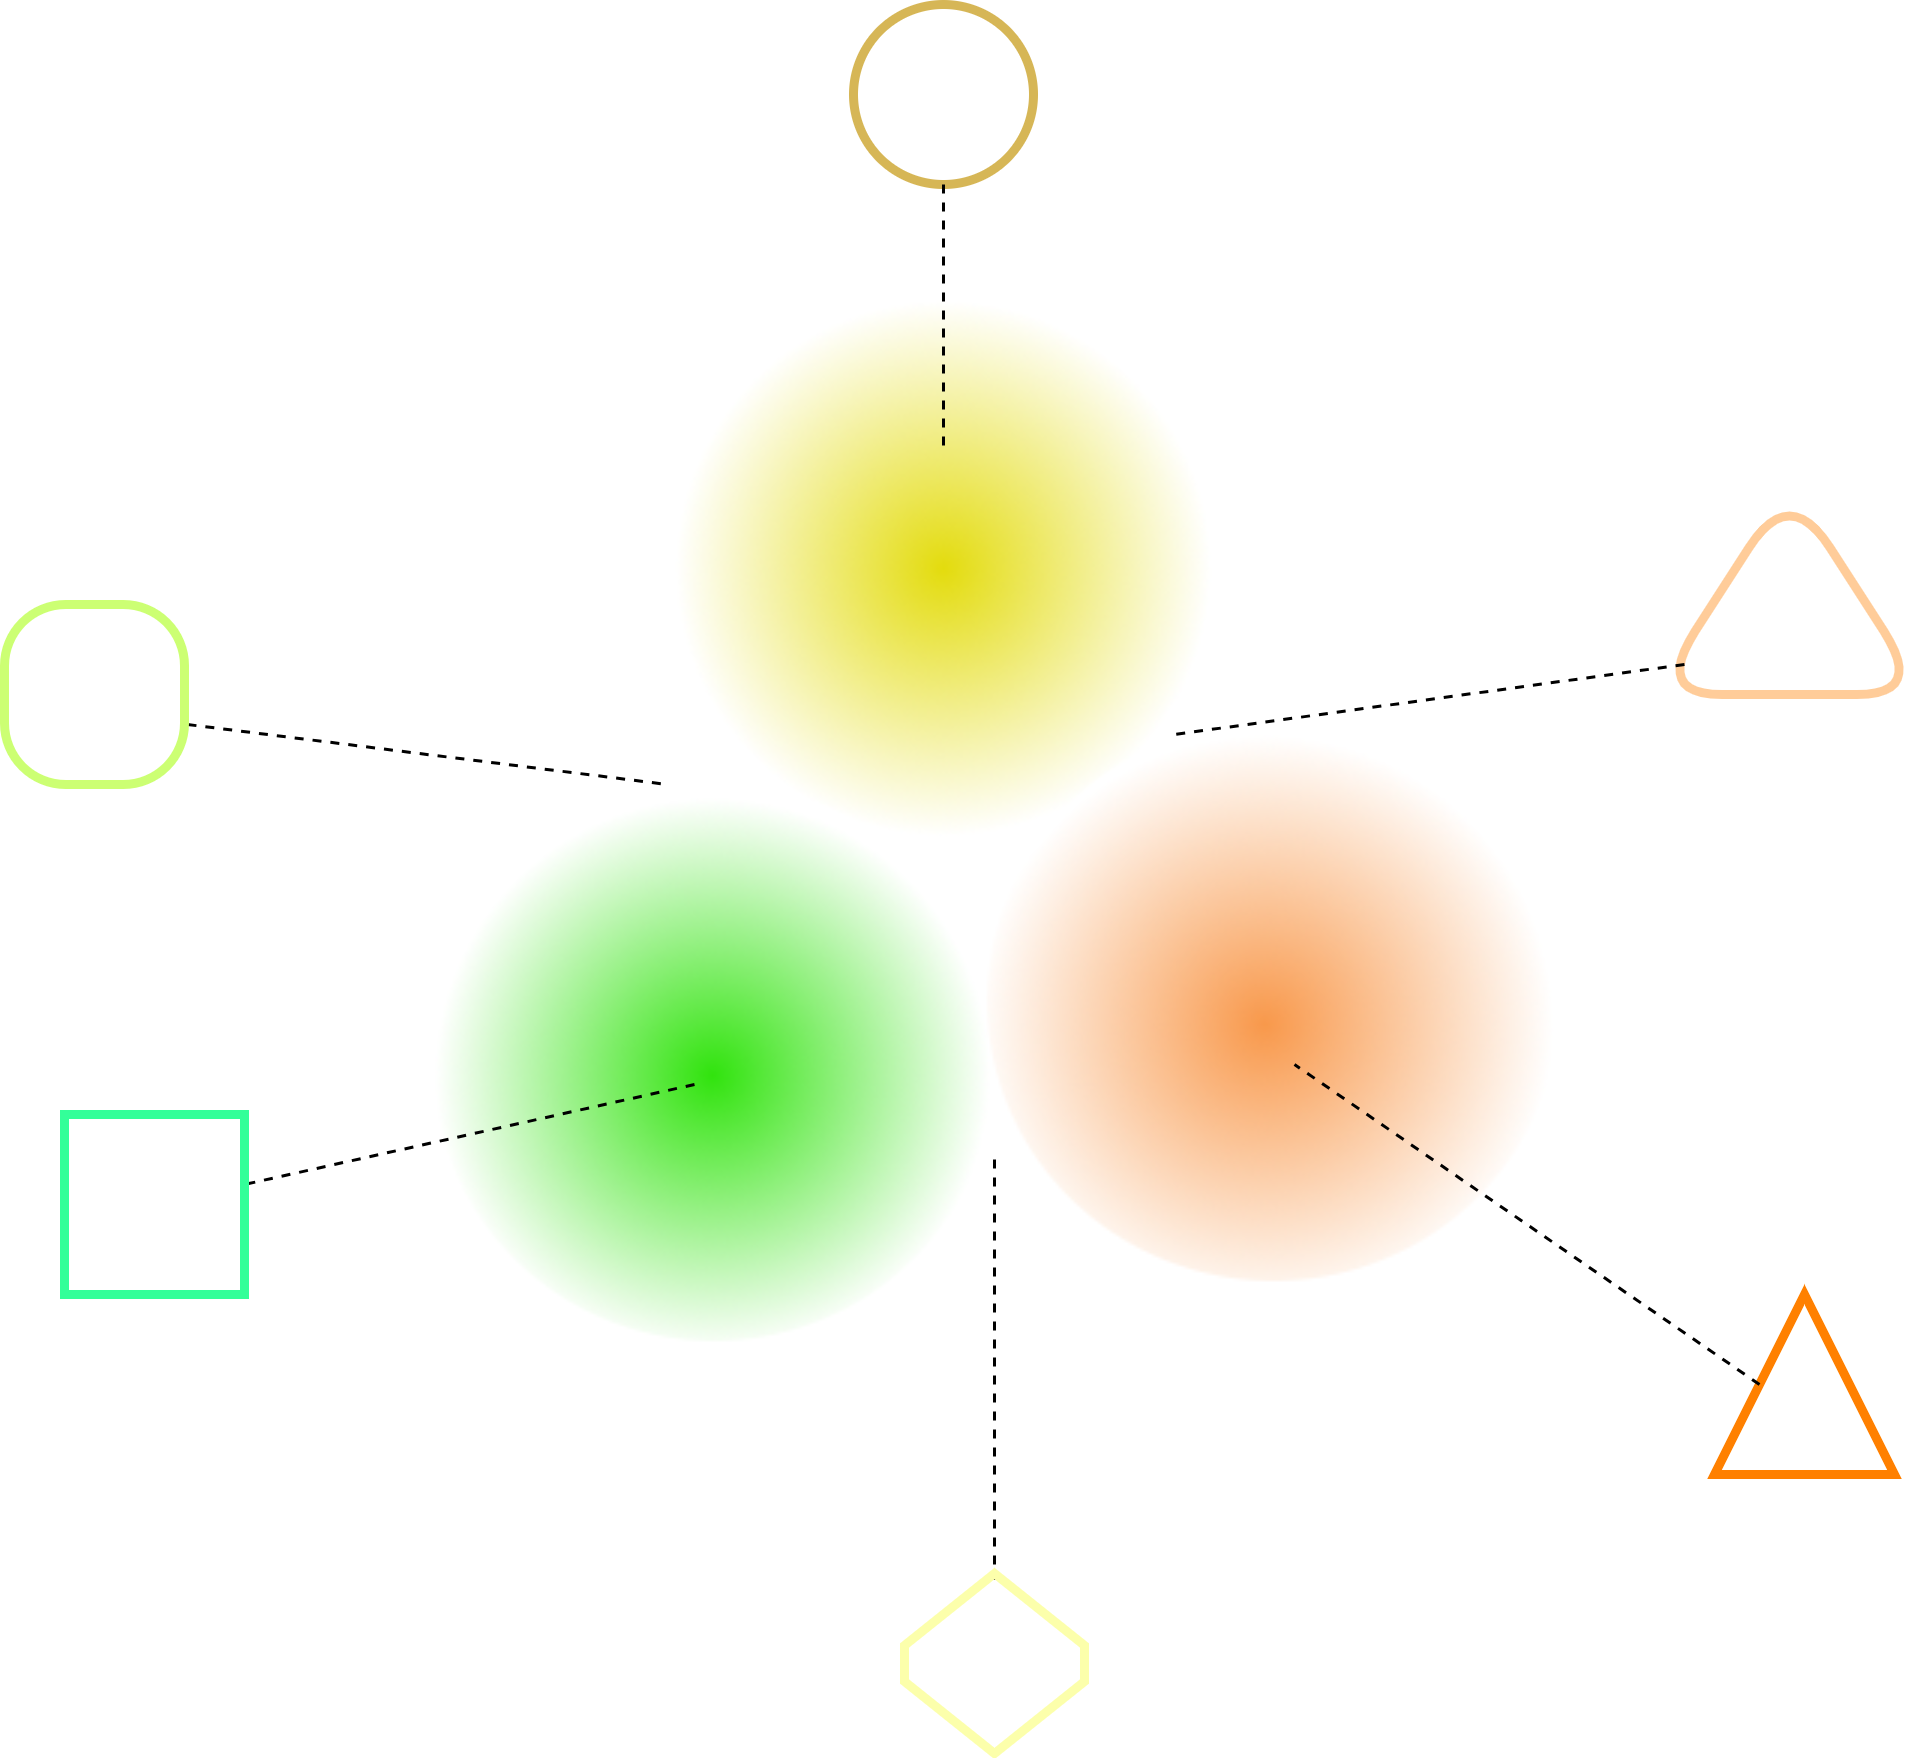
\includegraphics[width=0.46\textwidth]{images/VAE.png}
    \caption{Variational autoencoder latent space. The encoder distributions are distinguished by colors and different classes by shapes. It can be seen, the interpolation between two sampled points is meaningful}
    \label{fig:vae}
\end{figure}
Neural network training is a process during which the network learns to create internal representations of data in order to accomplish a given task.
In case of autoencoders, the task is to encode an input $\mathbf{x}$ in a way that allows for its reconstruction into the original form.
The autoencoder model consists of an encoder function $\varphi^{enc}$, which encodes an input $\mathbf{x}$ into a latent representation $\mathbf{z}$, and a decoder $\varphi^{dec}$, which models the conditional re-generation probability $p(\mathbf{x}|\mathbf{z})$.
In case of sequence autoencoders, both the encoder and decoder can be realized with an RNN.
However, vanilla autoencoders often fail to extract global semantic features of natural language sequences \cite{bowman2015generating}; therefore, adjustments need to be made in order to obtain better representations.
The technique proposed by \citet{kingma2013auto} uses the Variational Autoencoder (VAE) framework to tackle this issue.
The architecture is modified so that $\varphi^{enc}$ represents a recognition model $q(\mathbf{z}|\mathbf{x})$ which parameterizes an approximate posterior distribution over $\mathbf{z}$.
VAEs impose prior distribution on the latent variable $\mathbf{z}$, which acts as a regularization during training and makes it possible to draw samples from $q$.
Consequently, the VAE latent space is regular in a sense that it is possible to interpolate between two points.
The latent space structure is depicted schematically in Figure \ref{fig:vae}.
Typically, the modeled distributions are Gaussian and the prior is the standard normal distribution $N(0, 1)$.

We can realize the function modules in VAE using neural networks, however, there is a drawback regarding the implementation of sampling.
The sampling operation is not differentiable and therefore cannot be trained using standard approaches.
A solution to this problem is to use the \textit{reparameterization trick} \cite{kingma2013auto}.
The reparameterization trick uses the fact that a random variable under certain conditional distribution can be expressed as a deterministic transformation of some other variable with independent marginal distribution.
Distributions that allow us to do such a transformation include \textit{Gaussian, Logistic} or \textit{Gumbel}.

\paragraph{VAE latent space discretization}
Although VAE training yields robust representations that are also more interpretable thanks to the regularized latent space, in some cases, we require the latent representations to be discrete.
The motivation is mainly to improve interpretability and possibly uncover underlying processes in sequential tasks.
It is problematic to incorporate discrete variables into neural network models, because the widely used backpropagation algorithm requires smooth differentiable functions in order to propagate the gradients correctly.
\citet{van2017neural} propose a vector quantization technique to discretize the latent variables in VAEs.
Another approach is to use the the Gumbel-softmax distribution \cite{jang2016categorical} that enables us together with the reparameterization trick (Section \ref{sec:vae}) to work with categorical variables while not breaking the gradient flow in the network.

\paragraph{Variational Recurrent Neural Networks}
\label{sec:vrnn}
Variational Recurrent Neural Networks (VRNN) \cite{chung2015recurrent} explicitly model the dependencies between latent random variables across subsequent timesteps, similarly to dynamic Bayesian networks such as Hidden Markov Models (HMMs).
Unlike HMMs, the transitions between latent states are dependent not only on the state in the current time step, but also on the RNN hidden state which allows to model more complex dynamics.
Therefore, VRNNs are well suited for modeling sequential processes.
Basically, the VRNN is a recurrent network with a VAE in every time step.
The difference with respect to a basic VAE is that both prior and posterior distributions as well as the decoder are dependent on the RNN hidden state.
Formally, let $\mathbf{h}_{t}$ be the RNN hidden state in time step $t$.
The prior is realized with function $\varphi^{prior}(\mathbf{h}_{t-1})$, the posterior distribution $q$ is modeled with $\varphi^{enc}(\mathbf{x}_t, \mathbf{h}_{t-1})$ and the generation decoder distribution is $\varphi^{dec}(\mathbf{z}_t, \mathbf{h}_{t-1})$.

\section{Pretrained Language Models}
\subsection{\todo{}}
\begin{itemize}
    \item AuGPT - other experiments - using only portion of train set; compute number of training iterations; compare to RNNs
    \item LLM experiments
    \item Put it all together? is our NLU method able to improve performance of ZS LLMs/ latent models?
    \item Make work https://github.com/HLTCHKUST/Mem2Seq and look at the copy distributions
\end{itemize}

%
% TEXT END
%

\renewcommand{\chapterheadstartvskip}{\vspace*{0mm}} % chapter spacing

\cleardoublepage{}
\bibliographystyle{csplainnat}
\addcontentsline{toc}{chapter}{Bibliography}
{\small \bibliography{references,anthology}}

\cleardoublepage{}
\addcontentsline{toc}{chapter}{List of Abbreviations}
\renewcommand*{\acronymname}{List of Abbreviations}
\printglossary[type=\acronymtype,style=index]

\addcontentsline{toc}{chapter}{List of Tables}
{\small \listoftables\par}

\addcontentsline{toc}{chapter}{List of Figures}
{\small \listoffigures\par}

\cleardoublepage{}
\addcontentsline{toc}{chapter}{List of Publications}
\chapter*{List of Publications}

\phantom{\nobibliography*{references}}
\noindent We first present list of publications in which the author of this thesis is the main author, followed with more publications to which the author contributed. The number of citations was computed using Google Scholar.

Total number of citations: 112 


\vfill

% -----------------------------------------------------------------------------
\noindent\bibentry{hudecek-etal-2021-discovering}
\begin{itemize}[noitemsep,topsep=0pt]

\item This work presents pipeline method for unsupervised slot discovery.
\item Citations: 20

\end{itemize}\vspace{.5\baselineskip}

% -----------------------------------------------------------------------------
\noindent\bibentry{hudecek-dusek-2023-large}
\begin{itemize}[noitemsep,topsep=0pt]

\item In this work we use large language models and in-context learning to model task-oriented dialogue.

\item Citations: 8
\end{itemize}\vspace{.5\baselineskip}


% -----------------------------------------------------------------------------
\noindent\bibentry{hudecek-dusek-2022-learning}
\begin{itemize}[noitemsep,topsep=0pt]

\item In this publication we introduce our dialogue model with variational training and discrete latent space.
\item Citations: 1

\end{itemize}\vspace{.5\baselineskip}

% -----------------------------------------------------------------------------
\noindent\bibentry{hudecek-etal-2022-unifying}
\begin{itemize}[noitemsep,topsep=0pt]

\item In this work we present novel dialogue corpus and related experiments.
\item Citations: 0

\end{itemize}\vspace{.5\baselineskip}


% -----------------------------------------------------------------------------
\noindent\bibentry{kulhanek-etal-2021-augpt}
\begin{itemize}[noitemsep,topsep=0pt]

\item This work presents the AuGPT model and related experiments. It also describes the DSTC 8 challenge participation.
\item Citations: 44

\end{itemize}\vspace{.5\baselineskip}

% -----------------------------------------------------------------------------
\noindent\bibentry{straka-etal-2018-sumeczech}
\begin{itemize}[noitemsep,topsep=0pt]

\item This publication describes a dataset that can be used for training of summarization models of news in Czech language and related experiments.
\item Citations: 22

\end{itemize}\vspace{.5\baselineskip}

% -----------------------------------------------------------------------------
\noindent\bibentry{platek2016recurrent}
\begin{itemize}[noitemsep,topsep=0pt]

\item In this publication we introduce an RNN-based model used to dialogue state tracking as a sequence modeling task.

\item Citations: 11

\end{itemize}\vspace{.5\baselineskip}

% -----------------------------------------------------------------------------
\noindent\bibentry{schaub-etal-2021-definition}
\begin{itemize}[noitemsep,topsep=0pt]

\item This work discusses the inconsistencies and problems found in dialogue corpora
\item Citations: 5

\end{itemize}\vspace{.5\baselineskip}

% -----------------------------------------------------------------------------
\noindent\bibentry{mukherjee2023polite}
\begin{itemize}[noitemsep,topsep=0pt]

\item In this work we explore the abilities of language models for text style transfer.
\item Citations: 1

\end{itemize}\vspace{.5\baselineskip}

% -----------------------------------------------------------------------------
\noindent\bibentry{platek2023three}
\begin{itemize}[noitemsep,topsep=0pt]

\item In this work we propose ways of evaluating dialogue qualities with large language models and describe our submission to the DSTC 11 challenge.
\item Citations: 0

\end{itemize}\vspace{.5\baselineskip}

\end{document}
